\chapter{标量守恒律}
\label{chap:scalar-conservation-laws}

一条单行道上，前方路段车少、车开得快，后方路段车多、车开得慢。密度的分布会怎样随时间变化？第~\ref{chap:transport-equations}章的速度场是事先给定的，墨水只管被水流带走。车流不同：每辆车的速度取决于周围的密度，而密度又取决于所有车的位置。传播速度依赖未知量本身，这一点改变了全部局面。

最直接的后果是波形会变形。以一维Burgers方程为例，它的传播速度就等于场值：高处跑得快，低处跑得慢。高处从后面追上低处，波形的前沿越来越陡，到某一时刻斜率变成无穷，而场值始终有界。微分方程在这一刻失去了逐点的意义，路上的车却不会消失，区间内车辆总数的收支账依然成立。

于是要回到积分形式的收支平衡，并允许解带有间断。这一放宽有代价：同一个初值可以有无穷多个满足收支平衡的解，其中一个甚至让静止的流体自发运动起来。只算总账无法决定解，还需要一条规则来判定信息的传播方向。

本章沿着Burgers方程一路走下去。先用特征线算出光滑解何时失效，再写出允许间断的解和间断的传播速度，接着看选择规则怎样淘汰多余的解。把这些放到左右两个常状态的初值上，可以手算出两种基本的波。最后证明两个合乎规则的解的积分距离不会随时间增大，唯一性由此而来。

\section{守恒律问题}
\label{sec:cons-problem}

一段路上的车辆数只会因为有车从两端进出而改变。把这句话写成数学，就得到本章的方程。

\paragraph{从区间收支到方程}
设$u(x,t)$是$t$时刻$x$处的密度，例如单位长度上的车辆数。单位时间内向右穿过$x$点的量称为\term{通量}（flux）。本章假设通量只通过密度依赖位置和时间，写成$F(u(x,t))$，其中$F:\mathbb{R}\to\mathbb{R}$是给定的函数。

任取区间$[a,b]$，如图~\ref{fig:cons-balance}。区间内的总量只因两端的进出而变化，左端流入，右端流出：
\begin{equation}
  \frac{\mathrm{d}}{\mathrm{d}t}\int_a^b u(x,t)\,\mathrm{d}x=F(u(a,t))-F(u(b,t)).
  \label{eq:cons-balance}
\end{equation}

\begin{BookInlineFigure}
  \centering
  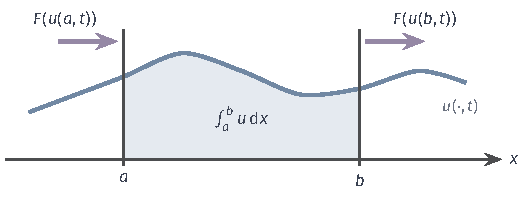
\includegraphics[width=89.8mm]{figures/06-differential-equations/02-partial-differential-equations/tikz/cons-balance/figure.pdf}
  \caption{区间上的收支。蓝线是某一时刻的密度$u(\cdot,t)$，浅蓝区域的面积是区间$[a,b]$内的总量。紫色箭头表示穿过两个端点的通量，左端流入增加总量，右端流出减少总量。}
  \label{fig:cons-balance}
\end{BookInlineFigure}

式~\eqref{eq:cons-balance}没有对$x$求导，也不要求$u$连续，只要积分和端点值有意义就能写出来。后面处理间断时正要回到这一点。现在先假设$u$和$F$都是$C^1$的，把右端写成$\partial_xF(u)$的积分：
\[
  \int_a^b\bigl(\partial_tu+\partial_xF(u)\bigr)\,\mathrm{d}x=0 .
\]

区间$[a,b]$是任取的，被积函数又连续。如果被积函数在某一点不为零，在该点附近的小区间上积分就不为零，与上式矛盾。于是得到
\begin{equation}
  \partial_tu+\partial_xF(u)=0,\qquad x\in\mathbb{R},\ t>0.
  \label{eq:cons-law}
\end{equation}

再给定初始分布
\begin{equation}
  u(x,0)=u_0(x),\qquad x\in\mathbb{R},
  \label{eq:cons-initial}
\end{equation}
式~\eqref{eq:cons-law}与~\eqref{eq:cons-initial}合起来就是\term{标量守恒律}（scalar conservation law）的初值问题。“守恒”一词来自式~\eqref{eq:cons-balance}：若$u$在无穷远处衰减，使两端的通量趋于同一个值，令$a\to-\infty$、$b\to\infty$，则右端为零，全直线上的总量$\int_{\mathbb{R}}u\,\mathrm{d}x$不随时间变化。

\paragraph{通量决定传播速度}
$C^1$解可以用链式法则展开$\partial_xF(u)$，得到
\begin{equation}
  \partial_tu+F'(u)\,\partial_xu=0.
  \label{eq:cons-quasilinear}
\end{equation}

把它与第~\ref{chap:transport-equations}章的输运方程$\partial_tu+v\,\partial_xu=0$对照，形式完全相同，只是速度$v$换成了$F'(u)$。$F'(u)$是密度$u$上的小扰动的传播速度。差别在于，输运方程的$v$事先已知，这里的速度要等解出$u$之后才知道。下面三种通量显示了通量形状带来的不同，见图~\ref{fig:cons-fluxes}。

\begin{itemize}
  \item 线性通量$F(u)=cu$：速度$F'(u)=c$是常数，方程退回到恒定速度的输运方程。
  \item \term{Burgers方程}（Burgers equation）的通量$F(u)=u^2/2$：速度$F'(u)=u$，场值本身就是传播速度。可以把$u$想成一维粒子各自的速度，每个粒子不受力，匀速前进。
  \item 车流通量$F(u)=u(1-u)$，其中$u\in[0,1]$是归一化密度：车速为$1-u$，空路上最快，堵死时为零，流量等于密度乘车速。
\end{itemize}

\begin{BookInlineFigure}
  \centering
  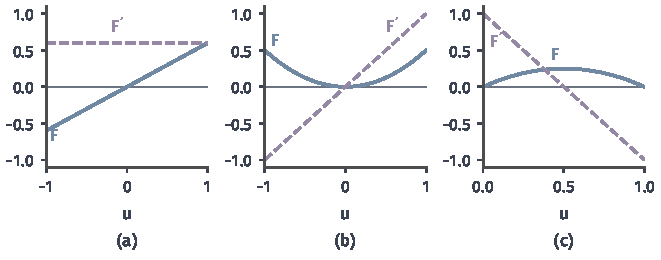
\includegraphics[width=112mm]{figures/06-differential-equations/02-partial-differential-equations/matplotlib/cons-fluxes/figure.pdf}
  \caption{三种通量及其传播速度。蓝色实线是通量$F$，紫色虚线是传播速度$F'$。(a)线性通量$F=0.6u$，速度为常数。(b)Burgers通量$F=u^2/2$，速度等于$u$，$F$是凸函数。(c)车流通量$F=u(1-u)$，速度$1-2u$随密度减小，$F$是凹函数。}
  \label{fig:cons-fluxes}
\end{BookInlineFigure}

车流的例子说明，扰动的传播速度和粒子的速度是两回事。取$u=3/4$，每辆车以速度$1-u=1/4$向前开，而密度扰动的传播速度是
\[
  F'(3/4)=1-2\cdot\frac34=-\frac12 ,
\]
它是负的。车在向前走，密度的变化却向后传，这就是堵车的尾部向后蔓延的原因。Burgers方程里两者恰好相同，读图和手算都最简单，所以本章用
\begin{equation}
  \partial_tu+\partial_x\Bigl(\frac{u^2}{2}\Bigr)=0
  \label{eq:cons-burgers}
\end{equation}
作贯穿全章的例子。

\paragraph{讨论的范围}
本章只讨论一维标量方程。未知量是向量的守恒律系统有多族速度不同的波，它们彼此耦合，本章后面的唯一性论证没有对应物。多维标量方程的熵解理论仍然成立，但间断不再是一条曲线，左右两侧的次序也不复存在，一维的显式构造不能照搬。下文的条件和结论都只针对一维标量问题。


\section{光滑解的失效}
\label{sec:cons-breakdown}

光滑解能活多久？特征线法可以回答这个问题：沿某条曲线把偏微分方程化成常微分方程。与第~\ref{chap:transport-equations}章的差别只在于曲线的速度依赖解。先假设$C^1$解存在，看它必须长什么样。

\paragraph{特征线是直线}
设$F\in C^2$，$u$是式~\eqref{eq:cons-law}的$C^1$解。从初始线上的点$(x_0,0)$出发，解常微分方程
\[
  x'(t)=F'\bigl(u(x(t),t)\bigr),\qquad x(0)=x_0 .
\]

沿这条曲线对$u$求导，再用式~\eqref{eq:cons-quasilinear}，得到
\[
  \frac{\mathrm{d}}{\mathrm{d}t}u(x(t),t)
  =\partial_tu+x'(t)\,\partial_xu
  =\partial_tu+F'(u)\,\partial_xu=0 .
\]

所以$u$沿曲线不变，始终等于$u_0(x_0)$。这样一来$x'(t)=F'(u_0(x_0))$是常数，曲线是一条直线。记
\begin{equation}
  a(x_0)=F'(u_0(x_0)),\qquad X_t(x_0)=x_0+a(x_0)\,t ,
  \label{eq:cons-characteristic}
\end{equation}
这些直线就是\term{特征线}（characteristic curve），$a(x_0)$是它的速度。解沿特征线保持常值：
\begin{equation}
  u\bigl(X_t(x_0),t\bigr)=u_0(x_0).
  \label{eq:cons-implicit}
\end{equation}

Burgers方程的$a=u_0$，特征线为$x=x_0+u_0(x_0)t$。下面的例子贯穿全章：
\begin{equation}
  u_0(x)=\frac{1}{1+x^2}.
  \label{eq:cons-bump}
\end{equation}

图~\ref{fig:cons-speed-arrows}把这条特征线翻译成波形的运动：曲线上的每个点水平移动，移动距离等于自己的高度。峰顶$x_0=0$、$u=1$的点在$t=1$移到$x=1$。右侧$x_0=2$、$u=1/5$的点只移到$x=2.2$。峰的右侧高处追赶低处，波形变陡；左侧高处离开低处，波形变缓。

\begin{BookInlineFigure}
  \centering
  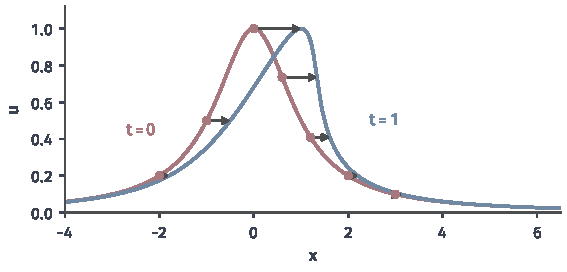
\includegraphics[width=96mm]{figures/06-differential-equations/02-partial-differential-equations/matplotlib/cons-speed-arrows/figure.pdf}
  \caption{Burgers方程中波形的水平移动。红线是初值~\eqref{eq:cons-bump}，红点是几个初始点，黑色箭头的长度等于该点的高度，蓝线是$t=1$的波形。峰的右侧被压陡，左侧被拉缓。}
  \label{fig:cons-speed-arrows}
\end{BookInlineFigure}

\paragraph{特征线相交与斜率爆炸}
斜率会变成多大？对式~\eqref{eq:cons-implicit}关于$x_0$求导，利用$\partial_{x_0}X_t=1+a'(x_0)t$，得到
\[
  \partial_xu\bigl(X_t(x_0),t\bigr)\,\bigl(1+a'(x_0)\,t\bigr)=u_0'(x_0).
\]

除过去，就是沿特征线的斜率公式：
\begin{equation}
  \partial_xu\bigl(X_t(x_0),t\bigr)=\frac{u_0'(x_0)}{1+a'(x_0)\,t}.
  \label{eq:cons-gradient}
\end{equation}

分母有直接的几何含义。$a'(x_0)$度量相邻特征线的速度差，两条相邻特征线的间距按因子$1+a'(x_0)t$变化。$a'<0$时，后面的特征线比前面的快，间距不断缩小；到$t=-1/a'(x_0)$，间距缩成零，分母为零，斜率发散。$a'>0$时间距增大，斜率随时间衰减。

在图~\ref{fig:cons-char-bump}中，初值峰右侧出发的特征线彼此靠拢，红色曲线是它们的包络，包络的尖点就是最早相交的位置。下面的例子算出这个点。

\begin{BookInlineFigure}
  \centering
  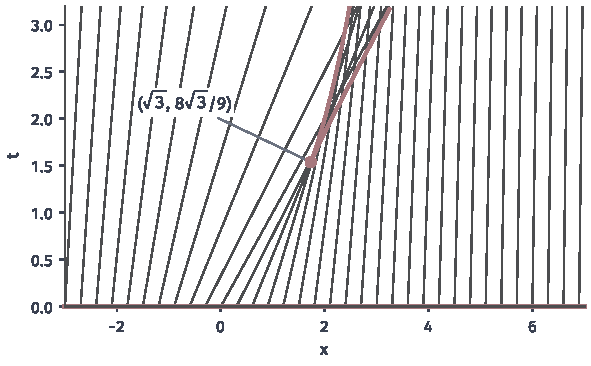
\includegraphics[width=100mm]{figures/06-differential-equations/02-partial-differential-equations/matplotlib/cons-char-bump/figure.pdf}
  \caption{初值~\eqref{eq:cons-bump}的特征线（深灰）。红色粗线是初始线，红色曲线是特征线的包络$t=-1/u_0'(x_0)$，$x=x_0+u_0(x_0)t$，它的尖点（红点）是特征线最早相交的位置。}
  \label{fig:cons-char-bump}
\end{BookInlineFigure}

\begin{example}[最早的相交点]
Burgers方程的$a=u_0$，取初值~\eqref{eq:cons-bump}。分母最早为零的特征线，出发点使$u_0'$最负。求导得
\[
  u_0'(x)=-\frac{2x}{(1+x^2)^2},\qquad u_0''(x)=\frac{6x^2-2}{(1+x^2)^3}.
\]

令$u_0''=0$，在$x>0$一侧得到$x_0=1/\sqrt{3}$。在这一点，
\[
  u_0(x_0)=\frac34,\qquad u_0'(x_0)=-\frac{2/\sqrt{3}}{(4/3)^2}=-\frac{3\sqrt{3}}{8}.
\]

于是最早的相交时刻和位置是
\[
  T^{*}=-\frac{1}{u_0'(x_0)}=\frac{8\sqrt{3}}{9}\approx1.54,\qquad
  x^{*}=x_0+\frac34T^{*}=\sqrt{3}.
\]
\end{example}

\paragraph{光滑解的寿命}
上面的计算是在假设解存在的前提下进行的。下面的定理确切地说明：相交时刻之前解存在且唯一，到了相交时刻不能再以$C^1$的方式继续。

\begin{theorem}[光滑解的寿命]
\label{thm:cons-lifespan}
设$F\in C^2(\mathbb{R})$，$u_0\in C^1(\mathbb{R})$，$u_0$与$u_0'$有界。记$a=F'\circ u_0$，$m=\inf_{\mathbb{R}}a'$。
\begin{enumerate}
  \item 若$m\geq0$，问题~\eqref{eq:cons-law}、\eqref{eq:cons-initial}在$\mathbb{R}\times[0,\infty)$上有唯一的$C^1$解。
  \item 若$m<0$，令
  \begin{equation}
    T^{*}=-\frac{1}{m},
    \label{eq:cons-breaking-time}
  \end{equation}
  此时问题在时间段$[0,T^{*})$上有唯一的$C^1$解，解的值保持在$[\inf u_0,\sup u_0]$内。当$t\uparrow T^{*}$时，$\sup_x\lvert\partial_xu(x,t)\rvert\to\infty$。对任何$T>T^{*}$，$\mathbb{R}\times[0,T]$上不存在$C^1$解；若下确界$m$在某点取到，$T=T^{*}$时同样不存在。
\end{enumerate}
\end{theorem}

\begin{proof}
记$T_0=\infty$（$m\geq0$时）或$T_0=T^{*}$（$m<0$时）。先看映射$X_t$。对$0\leq t<T_0$，
\[
  \partial_{x_0}X_t=1+a'(x_0)\,t\geq1+\min(m,0)\,t>0 .
\]
导数有正的下界，所以$X_t$严格递增，且把$\mathbb{R}$映满$\mathbb{R}$，是$C^1$同胚。

唯一性：设$u$是$\mathbb{R}\times[0,T_0)$上的$C^1$解。前面已经说明，$u$沿式~\eqref{eq:cons-characteristic}的直线不变。这些直线在$t$时刻覆盖整条实轴，所以$u$的值被式~\eqref{eq:cons-implicit}完全确定。

存在性：令$\xi(x,t)$是方程$X_t(\xi)=x$的解。由隐函数定理，$\xi\in C^1$，并且
\[
  \partial_x\xi=\frac{1}{1+a'(\xi)\,t},\qquad
  \partial_t\xi=-\frac{a(\xi)}{1+a'(\xi)\,t}.
\]

定义$u(x,t)=u_0(\xi(x,t))$。它在$t=0$取$u_0$，并且$F'(u)=a(\xi)$，所以
\[
  \partial_tu+F'(u)\,\partial_xu
  =u_0'(\xi)\bigl(\partial_t\xi+a(\xi)\,\partial_x\xi\bigr)=0 .
\]
第一条结论与第二条的存在性就此成立。$u$的值都是$u_0$的值，所以落在$[\inf u_0,\sup u_0]$内。

斜率发散：设$m<0$。取点列$x_n$使$a'(x_n)\to m$。记$C=\max\lvert F''\rvert$，最大值取在$u_0$值域的闭包上，它是紧集，且$C>0$（否则$a'\equiv0$）。由$a'=F''(u_0)u_0'$，当$n$充分大时
\[
  \lvert u_0'(x_n)\rvert\geq\frac{\lvert a'(x_n)\rvert}{C}\geq\frac{\lvert m\rvert}{2C}.
\]

对固定的$t<T^{*}$，有$1+mt>0$，且$n\to\infty$时$1+a'(x_n)t\to1+mt$。取$n$充分大，使$1+a'(x_n)t\leq2(1+mt)$，由式~\eqref{eq:cons-gradient}，
\[
  \sup_x\lvert\partial_xu(x,t)\rvert\geq\frac{\lvert m\rvert}{4C\,(1+mt)}.
\]
令$t\uparrow T^{*}$，右端趋于无穷。

不可延拓：设$u$是$\mathbb{R}\times[0,T]$上的$C^1$解，$T>T^{*}$。由$m<-1/T$，存在$x_0$使$a'(x_0)<-1/T$；若下确界在某点取到且$T=T^{*}$，就取该点。令$t_1=-1/a'(x_0)\in(0,T]$，此时$a'(x_0)\neq0$，从而$u_0'(x_0)\neq0$。

前面的推导对解存在的整个时间段成立，于是在$t=t_1$时
\[
  \partial_xu\bigl(X_{t_1}(x_0),t_1\bigr)\,\bigl(1+a'(x_0)\,t_1\bigr)=u_0'(x_0).
\]
左端的第二个因子为零，右端不为零，矛盾。
\end{proof}

对Burgers方程，$a'=u_0'$，$T^{*}=-1/\inf u_0'$。特别地，有界的$C^1$初值（导数有界）给出整体$C^1$解，当且仅当$u_0$单调不减。定理中的条件各有作用：$u_0'$有界保证$m$有限，否则$T^{*}$可以为零；$F''$非零才让速度随$u$变化，线性通量的$a'\equiv0$，永远不会相交。

有界性和光滑性是分开的两件事。第~\ref{chap:ordinary-differential-equations}章的爆炸是解的值趋于无穷；这里相反，解的值始终在初值范围内，发散的是导数。图~\ref{fig:cons-gradient-blowup}显示，初值~\eqref{eq:cons-bump}的压缩侧斜率在$T^{*}$发散，膨胀侧斜率逐渐衰减，而最大值始终为$1$。

\begin{BookInlineFigure}
  \centering
  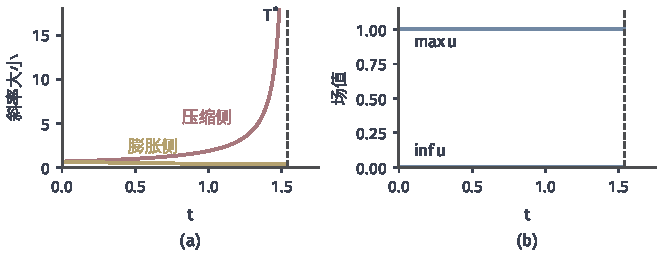
\includegraphics[width=112mm]{figures/06-differential-equations/02-partial-differential-equations/matplotlib/cons-gradient-blowup/figure.pdf}
  \caption{初值~\eqref{eq:cons-bump}的斜率与场值。(a)红线是压缩侧的最大下降斜率$\max_{x_0}(-u_0'/(1+tu_0'))$，黄线是膨胀侧的最大上升斜率，虚线是$T^{*}$。(b)场值的上界和下确界（蓝）不随时间变化。}
  \label{fig:cons-gradient-blowup}
\end{BookInlineFigure}

\paragraph{相交之后发生了什么}
定理说的是映射$X_t$的单调性。图~\ref{fig:cons-fold-map}画出$x_0\mapsto X_t(x_0)$在三个时刻的形状：$T^{*}$之前严格递增，$T^{*}$时出现水平切点，之后出现折叠，同一个$x$有三个原像，也就是有三条特征线到达同一点，各自带来不同的值。

\begin{BookInlineFigure}
  \centering
  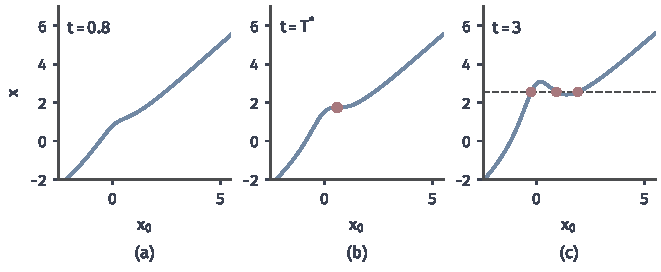
\includegraphics[width=112mm]{figures/06-differential-equations/02-partial-differential-equations/matplotlib/cons-fold-map/figure.pdf}
  \caption{初值~\eqref{eq:cons-bump}的映射$X_t$。(a)$t=0.8$，严格递增。(b)$t=T^{*}$，红点是水平切点$(1/\sqrt{3},\sqrt{3})$。(c)$t=3$，映射折叠，虚线$x=2.55$与曲线有三个交点（红点）。}
  \label{fig:cons-fold-map}
\end{BookInlineFigure}

把折叠的结果画成波形，就是图~\ref{fig:cons-steepening}(b)：曲线翻转，成为多值的。水面的波可以卷起来，同一个$x$上有几层水；密度却不能，同一时刻同一地点只有一个车流密度。所以$T^{*}$之后，式~\eqref{eq:cons-implicit}不再给出一个函数。

\begin{BookInlineFigure}
  \centering
  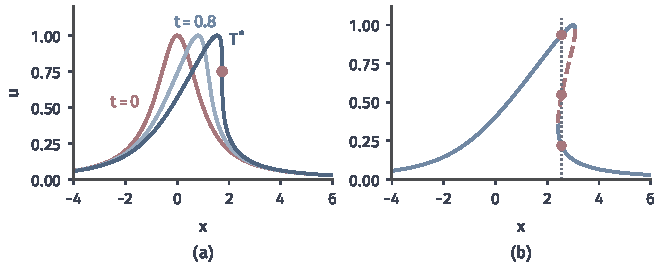
\includegraphics[width=112mm]{figures/06-differential-equations/02-partial-differential-equations/matplotlib/cons-steepening/figure.pdf}
  \caption{波形的变陡与翻转。(a)红线是$t=0$，蓝色由浅到深是$t=0.8$和$t=T^{*}$，红点是斜率首次为无穷的位置$(\sqrt{3},3/4)$。(b)$t=3$时沿特征线算出的图像，红色虚线是翻转部分，竖直点线$x=2.55$上有三个值。}
  \label{fig:cons-steepening}
\end{BookInlineFigure}

第~\ref{chap:transport-equations}章的轨迹不会相交，原因是给定的Lipschitz速度场让常微分方程的解唯一，两条轨迹不能在同一时刻到达同一点。这里两条特征线到达同一点时带着不同的场值，也就有不同的速度，它们不是同一个速度场下的轨迹，唯一性定理管不到它们。速度依赖解，正是相交的来源。

\paragraph{斜坡：所有特征线同时汇聚}
还有一个算起来更简单的初值：
\begin{equation}
  u_0(x)=\begin{cases}1,&x<0,\\1-x,&0\leq x\leq1,\\0,&x>1.\end{cases}
  \label{eq:cons-ramp}
\end{equation}

它只是Lipschitz连续，但沿特征线的计算不受影响。在$(0,1)$上$a'=-1$，从那里出发的特征线$x=x_0+(1-x_0)t$全部在$(1,1)$汇聚，$T^{*}=1$。反解出$x_0=(x-t)/(1-t)$，得到$t<1$时的解
\begin{equation}
  u(x,t)=\frac{1-x}{1-t},\qquad t\leq x\leq1,
  \label{eq:cons-ramp-solution}
\end{equation}
其余区域取常值$1$或$0$。第~\ref{sec:cons-weak}节将接着算出$t>1$时的解，这时解必须带一个间断。


\section{弱解}
\label{sec:cons-weak}

特征线在$T^{*}$失效，收支平衡并没有失效。路上的车不会因为斜率变成无穷而消失，式~\eqref{eq:cons-balance}依然有意义。我们需要一种不依赖导数的方式说出“解满足方程”，并回答间断会以多快的速度移动。

\subsection{积分守恒}
\label{subsec:cons-integral}

把式~\eqref{eq:cons-balance}对时间从$t_1$积分到$t_2$，得到时空矩形上的收支账：
\begin{equation}
  \begin{aligned}
    &\int_a^b u(x,t_2)\,\mathrm{d}x-\int_a^b u(x,t_1)\,\mathrm{d}x\\
    &\qquad+\int_{t_1}^{t_2}F(u(b,t))\,\mathrm{d}t
    -\int_{t_1}^{t_2}F(u(a,t))\,\mathrm{d}t=0 .
  \end{aligned}
  \label{eq:cons-box}
\end{equation}

图~\ref{fig:cons-box}把四项画在$(x,t)$平面上：矩形的上下两边记录总量，左右两边记录流过的量。把$(F(u),u)$看成$(x,t)$平面上的向量场，式~\eqref{eq:cons-box}说的是这个场穿过矩形边界的净通量为零。间断线可以从矩形中穿过，这四项仍然都有意义。

\begin{BookInlineFigure}
  \centering
  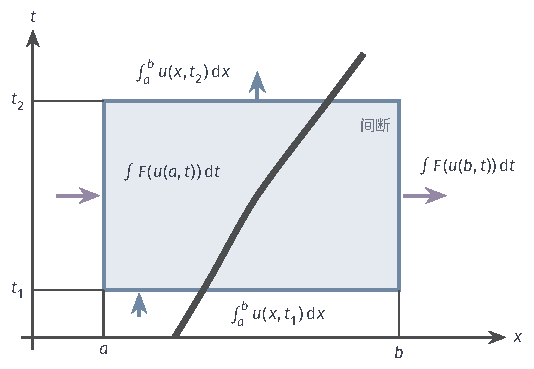
\includegraphics[width=90.4mm]{figures/06-differential-equations/02-partial-differential-equations/tikz/cons-box/figure.pdf}
  \caption{时空矩形上的收支。上下两边的蓝色箭头记录$t_2$、$t_1$时刻区间内的总量，左右两边的紫色箭头记录时段内流入、流出的量。深灰粗线是一条间断线，它穿过矩形时四项仍有定义。}
  \label{fig:cons-box}
\end{BookInlineFigure}

\paragraph{用光滑权重代替矩形}
用矩形检验有两点不便：它要用到$u$在线段上的值，而$u$只是有界可测时这样的值没有确切含义；矩形的边角也不便做微积分。办法是把矩形的示性函数换成光滑的权重$\varphi$，如图~\ref{fig:cons-test-weight}。这就像用一个边缘柔和的窗口观察收支，$\varphi$在窗口内部几乎是常数，它的导数集中在边缘附近，而边缘正是收支发生的地方。

\begin{BookInlineFigure}
  \centering
  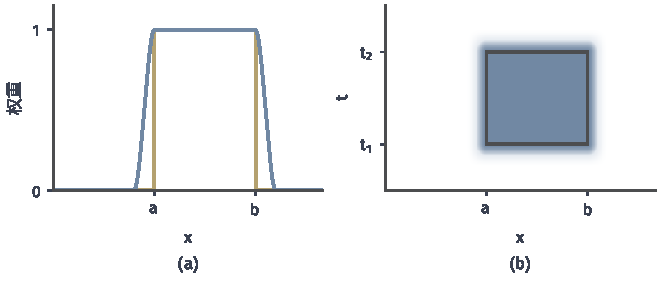
\includegraphics[width=112mm]{figures/06-differential-equations/02-partial-differential-equations/matplotlib/cons-test-weight/figure.pdf}
  \caption{用光滑权重代替矩形。(a)一维剖面：黄线是示性函数，蓝线是光滑的近似。(b)时空平面上的权重$\varphi$，颜色越深值越大，黑框是矩形$[a,b]\times[t_1,t_2]$。$\varphi$的导数只在黑框附近不为零。}
  \label{fig:cons-test-weight}
\end{BookInlineFigure}

设$u$是$C^1$解，$\varphi\in C_c^{\infty}(\mathbb{R}\times[0,\infty))$是\term{测试函数}（test function）。它在$t=0$可以不为零，在大的$\lvert x\rvert$和$t$上为零。把式~\eqref{eq:cons-law}乘以$\varphi$再积分：
\[
  \int_0^{\infty}\!\!\int_{\mathbb{R}}\bigl(\partial_tu+\partial_xF(u)\bigr)\varphi\,\mathrm{d}x\,\mathrm{d}t=0 .
\]

对$t$分部积分时，下限$t=0$留下一项$-\int_{\mathbb{R}}u_0\,\varphi(\cdot,0)\,\mathrm{d}x$；对$x$分部积分没有边界项。所有导数都转到$\varphi$上之后，得到下面的定义。

\begin{definition}[弱解]
\label{def:cons-weak-solution}
设$u_0\in L^{\infty}(\mathbb{R})$，$F\in C^1(\mathbb{R})$。有界可测函数$u$称为问题~\eqref{eq:cons-law}、\eqref{eq:cons-initial}的\term{弱解}（weak solution），若对每个$\varphi\in C_c^{\infty}(\mathbb{R}\times[0,\infty))$，
\begin{equation}
  \int_0^{\infty}\!\!\int_{\mathbb{R}}\bigl(u\,\partial_t\varphi+F(u)\,\partial_x\varphi\bigr)\,\mathrm{d}x\,\mathrm{d}t
  +\int_{\mathbb{R}}u_0\,\varphi(\cdot,0)\,\mathrm{d}x=0 .
  \label{eq:cons-weak}
\end{equation}
\end{definition}

式~\eqref{eq:cons-weak}没有$u$的导数，间断的$u$也能代入。初值的进入方式值得留意：$\varphi$在$t=0$不必为零，第二项正是下边界上的收支。若只取在$t=0$附近为零的$\varphi$，初值就看不见了。

取$\varphi$趋于矩形的示性函数，$\partial_t\varphi$在矩形上下边附近集中，$\partial_x\varphi$在左右边附近集中，式~\eqref{eq:cons-weak}的极限就回到式~\eqref{eq:cons-box}，对几乎所有的$a,b,t_1,t_2$成立。弱形式与矩形收支说的是同一件事。

弱解的概念确实推广了经典解，下面的引理说明两者在光滑情形下一致。

\begin{lemma}[经典解与弱解]
\label{lem:cons-classical-weak}
设$u\in C^1(\mathbb{R}\times[0,\infty))$有界，$F\in C^1$，$u_0$连续有界。则$u$是经典解（满足式~\eqref{eq:cons-law}、\eqref{eq:cons-initial}）当且仅当$u$满足式~\eqref{eq:cons-weak}。
\end{lemma}

\begin{proof}
必要性就是上面的分部积分。

充分性：式~\eqref{eq:cons-weak}对$u$反向分部积分。先取在$t=0$附近为零的$\varphi$，得到
\[
  \int_0^{\infty}\!\!\int_{\mathbb{R}}\bigl(\partial_tu+\partial_xF(u)\bigr)\varphi\,\mathrm{d}x\,\mathrm{d}t=0 .
\]
被积函数中的括号连续，若在某点不为零，取该点附近符号一致的$\varphi\geq0$，积分不为零，矛盾。所以式~\eqref{eq:cons-law}处处成立。

再取一般的$\varphi$，反向分部积分后内部的项已经为零，剩下
\[
  \int_{\mathbb{R}}\bigl(u_0-u(\cdot,0)\bigr)\varphi(\cdot,0)\,\mathrm{d}x=0 .
\]
$\varphi(\cdot,0)$可以是任意的$C_c^{\infty}$函数，所以$u(\cdot,0)=u_0$。
\end{proof}

\paragraph{分段满足方程并不够}
弱形式放宽了要求，但并非什么间断都行。取初值$u_0=1$（$x<0$）、$u_0=0$（$x>0$）。候选函数“间断永远不动”，即$u(x,t)=u_0(x)$，在间断线两侧都是常数，逐点满足方程。

用式~\eqref{eq:cons-box}在矩形$[-1,1]\times[0,1]$上算账，见图~\ref{fig:cons-wrong-speed}(a)。区间内的总量两个时刻都是$1$，变化量为零。左端流入$F(1)\cdot1=1/2$，右端流出$F(0)\cdot1=0$，净流入为$1/2$。账对不上，因为流进来的$1/2$没有地方去。

如果间断以速度$1/2$右移，$t=1$时总量变成$3/2$，增加的$1/2$恰好是净流入，账就平了，见图~\ref{fig:cons-wrong-speed}(b)。可见分段满足方程还不够，间断的移动速度必须与流入流出相配。下一小节给出这个条件。

\begin{BookInlineFigure}
  \centering
  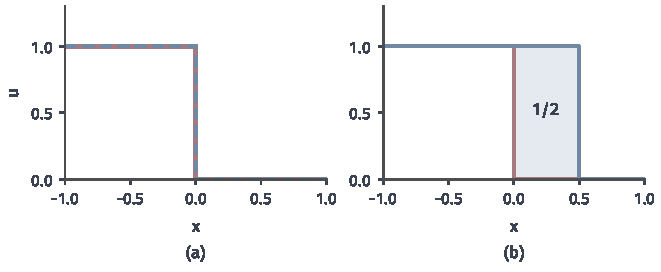
\includegraphics[width=112mm]{figures/06-differential-equations/02-partial-differential-equations/matplotlib/cons-wrong-speed/figure.pdf}
  \caption{间断速度与收支账，初值为左$1$右$0$的阶跃（红），$t=1$时的候选解为蓝线。(a)间断不动：总量不变，净流入的$1/2$无处安放。(b)间断以速度$1/2$右移：浅蓝矩形的面积$1/2$恰好等于净流入。}
  \label{fig:cons-wrong-speed}
\end{BookInlineFigure}

\paragraph{收支账选不出解}
反过来，把收支账算平也未必就够了。取Burgers方程和相反的阶跃：$u_0=0$（$x<0$）、$u_0=1$（$x>0$）。下面两个函数的初值都是这个阶跃：
\[
  u^{\mathrm{j}}(x,t)=\begin{cases}0,&x<t/2,\\1,&x>t/2,\end{cases}\qquad
  u^{\mathrm{f}}(x,t)=\begin{cases}0,&x\leq0,\\x/t,&0<x<t,\\1,&x\geq t.\end{cases}
\]

在矩形$[-2,2]\times[0,1]$上算账。初始总量是$2$，右端流出$F(1)\cdot1=1/2$，左端不流入，所以$t=1$时总量应为$3/2$。对$u^{\mathrm{j}}$，$t=1$时值为$1$的部分长度是$3/2$；对$u^{\mathrm{f}}$，总量是
\[
  \int_0^1x\,\mathrm{d}x+1\cdot1=\frac32 .
\]
两个账都平，差别只是把图~\ref{fig:cons-same-ledger}中两块面积相等的小三角形互换了位置。

\begin{BookInlineFigure}
  \centering
  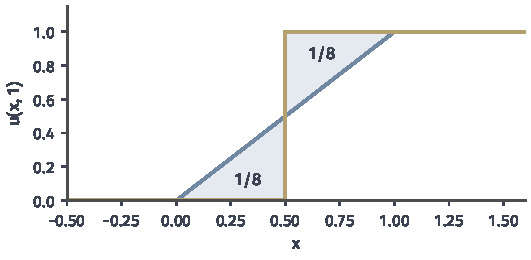
\includegraphics[width=90mm]{figures/06-differential-equations/02-partial-differential-equations/matplotlib/cons-same-ledger/figure.pdf}
  \caption{同一阶跃初值的两个候选解在$t=1$的形状：黄线是带间断的$u^{\mathrm{j}}$，蓝线是连续的$u^{\mathrm{f}}$。两块浅蓝三角形的面积都是$1/8$，一增一减，总量相同。}
  \label{fig:cons-same-ledger}
\end{BookInlineFigure}

矩形收支是必要条件，这里只验证了一个矩形。下一小节的定理会说明这两个函数确实都是弱解。经典解一定满足弱形式，但弱形式可以容许同一个初值有多个解，这是放宽解的概念要付的代价。

\subsection{跳跃条件}
\label{subsec:cons-jump}

间断以多快的速度移动？设间断两侧的状态是$u_-$（左）和$u_+$（右），间断的速度是$s$。

换到跟着间断一起运动的坐标系，见图~\ref{fig:cons-moving-jump}(b)。在这个坐标系里间断静止，所有物质的速度都减去了$s$，通量相应变成$F(u)-su$。间断是一条线，存不下任何东西，所以从左边进入的量必须等于从右边流出的量：
\[
  F(u_-)-s\,u_-=F(u_+)-s\,u_+ .
\]

\begin{BookInlineFigure}
  \centering
  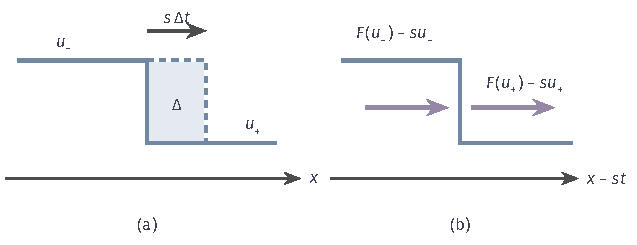
\includegraphics[width=107.9mm]{figures/06-differential-equations/02-partial-differential-equations/tikz/cons-moving-jump/figure.pdf}
  \caption{间断处的收支。(a)实验室坐标：时间$\Delta t$内间断移动$s\Delta t$，浅蓝矩形内的总量变化$(u_--u_+)s\Delta t$必须等于净流入。(b)随间断运动的坐标：相对通量$F(u)-su$在间断两侧相等，紫色箭头表示这两股流量。}
  \label{fig:cons-moving-jump}
\end{BookInlineFigure}

移项就得到\term{Rankine--Hugoniot条件}（Rankine--Hugoniot condition）。下面的定理说明，这个条件恰好刻画了分段光滑函数何时是弱解。

\begin{theorem}[Rankine--Hugoniot条件]
\label{thm:cons-rh}
设$F\in C^1$，$V\subset\mathbb{R}\times(0,\infty)$是开集，$C^1$曲线$x=\gamma(t)$把$V$分成左右两部分$V_-$、$V_+$。设$u$在$V_\pm$内是$C^1$的并满足式~\eqref{eq:cons-law}，$u$及其一阶偏导都能连续延拓到曲线的两侧，单侧极限记为$u_\pm(t)$。则$u$对所有$\varphi\in C_c^{\infty}(V)$满足
\begin{equation}
  \iint_V\bigl(u\,\partial_t\varphi+F(u)\,\partial_x\varphi\bigr)\,\mathrm{d}x\,\mathrm{d}t=0
  \label{eq:cons-rh-weak}
\end{equation}
当且仅当在曲线上
\begin{equation}
  \gamma'(t)\,\bigl(u_+-u_-\bigr)=F(u_+)-F(u_-).
  \label{eq:cons-rh}
\end{equation}
\end{theorem}

\begin{proof}
考虑$(x,t)$平面上的向量场$\bm{W}=(F(u)\varphi,\ u\varphi)$。在$V_\pm$内，利用式~\eqref{eq:cons-law}，
\[
  \nabla_{(x,t)}\cdot\bm{W}=F(u)\,\partial_x\varphi+u\,\partial_t\varphi .
\]

$\varphi$在$V$的边界附近为零，所以在$V_-$上用散度定理时，只有曲线部分有贡献。曲线$x-\gamma(t)=0$上指向$V_+$（即$V_-$的外法向）的方向是$(1,-\gamma')$，弧长元是$\sqrt{1+\gamma'^2}\,\mathrm{d}t$，单位化因子抵消，于是
\[
  \iint_{V_-}\bigl(u\,\partial_t\varphi+F(u)\,\partial_x\varphi\bigr)\,\mathrm{d}x\,\mathrm{d}t
  =\int\bigl(F(u_-)-\gamma'u_-\bigr)\,\varphi(\gamma(t),t)\,\mathrm{d}t .
\]

在$V_+$上外法向反号，得到
\[
  \iint_{V_+}\bigl(u\,\partial_t\varphi+F(u)\,\partial_x\varphi\bigr)\,\mathrm{d}x\,\mathrm{d}t
  =-\int\bigl(F(u_+)-\gamma'u_+\bigr)\,\varphi(\gamma(t),t)\,\mathrm{d}t .
\]

两式相加，积分等式等价于
\[
  \int\Bigl(F(u_-)-F(u_+)-\gamma'(u_--u_+)\Bigr)\,\varphi(\gamma(t),t)\,\mathrm{d}t=0
\]
对所有$\varphi$成立。括号里的函数连续，$\varphi$在曲线上的值可以任取，所以这等价于括号恒为零，即式~\eqref{eq:cons-rh}。
\end{proof}

定理针对$t>0$的内部。若分段$C^1$的$u$在各块上取到相应的初值，边界$t=0$的项恰好给出式~\eqref{eq:cons-weak}中的初值积分，所以$u$是弱解当且仅当每条间断线上式~\eqref{eq:cons-rh}成立。有两个特殊情形要留意。$u_+=u_-$时式~\eqref{eq:cons-rh}自动成立，所以$u$连续、仅导数间断的折线不需要额外条件，前面的$u^{\mathrm{f}}$就属于这种情形。条件的另一面是，它只约束速度，不约束两侧状态的相对大小。

\paragraph{波速是通量的弦斜率}
$u_-\neq u_+$时，式~\eqref{eq:cons-rh}给出
\begin{equation}
  s=\frac{F(u_+)-F(u_-)}{u_+-u_-},
  \label{eq:cons-shock-speed}
\end{equation}
它是通量图像上连接两个状态的弦的斜率，如图~\ref{fig:cons-rh-chord}。由积分中值定理，$s$是$F'$在$u_-$与$u_+$之间的平均值。Burgers方程的弦斜率特别简单：
\begin{equation}
  s=\frac{u_-+u_+}{2}.
  \label{eq:cons-burgers-speed}
\end{equation}
前面的阶跃取$u_-=0$、$u_+=1$，$s=1/2$，所以$u^{\mathrm{j}}$确实是弱解；$u^{\mathrm{f}}$由两条连续接缝组成，也是弱解。一个初值，两个弱解。

\begin{BookInlineFigure}
  \centering
  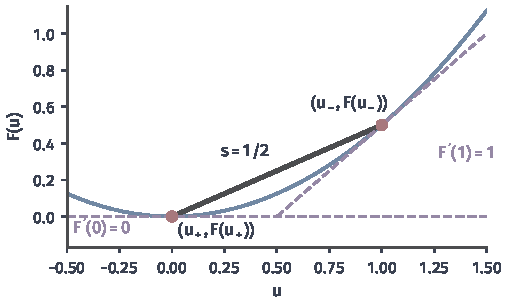
\includegraphics[width=86mm]{figures/06-differential-equations/02-partial-differential-equations/matplotlib/cons-rh-chord/figure.pdf}
  \caption{Rankine--Hugoniot速度的几何含义，$F=u^2/2$（蓝）。两个红点是状态$u_-=1$、$u_+=0$，深灰粗线是弦，斜率$s=1/2$。紫色虚线是两端的切线，斜率$F'(1)=1$与$F'(0)=0$，$s$介于两者之间。}
  \label{fig:cons-rh-chord}
\end{BookInlineFigure}

\paragraph{斜坡初值的后续}
现在可以接着算斜坡~\eqref{eq:cons-ramp}。$t=1$时解变成左$1$右$0$的台阶，位置在$x=1$。此后沿用这个台阶，令间断从$(1,1)$出发，由式~\eqref{eq:cons-burgers-speed}，速度是$1/2$，于是间断线为$x=(1+t)/2$，解为
\begin{equation}
  u(x,t)=\begin{cases}1,&x<(1+t)/2,\\0,&x>(1+t)/2,\end{cases}\qquad t\geq1.
  \label{eq:cons-ramp-shock}
\end{equation}

图~\ref{fig:cons-ramp-shock}(a)中，左侧的特征线以速度$1$从后面追上间断，右侧的特征线停在原地等间断到来，都终止在间断线上。

\begin{BookInlineFigure}
  \centering
  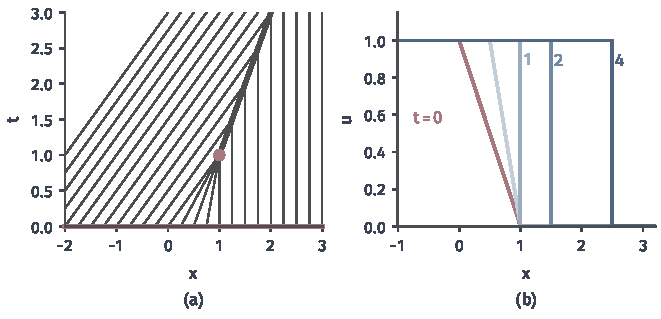
\includegraphics[width=112mm]{figures/06-differential-equations/02-partial-differential-equations/matplotlib/cons-ramp-shock/figure.pdf}
  \caption{斜坡初值的解。(a)特征线（细线）在红点$(1,1)$汇聚，此后深灰粗线$x=(1+t)/2$是间断线，两侧的特征线都在它上面终止。(b)红线是$t=0$，蓝色由浅到深是$t=0.5,1,2,4$。}
  \label{fig:cons-ramp-shock}
\end{BookInlineFigure}

\paragraph{等面积法则}
式~\eqref{eq:cons-ramp-shock}还可以换一个角度得到。沿特征线得到的多值图像虽然不是函数，但曲线下的面积是守恒的。把图像写成参数形式$(x_0+tu_0(x_0),\,u_0(x_0))$，带符号的面积随时间的变化是
\[
  \frac{\mathrm{d}}{\mathrm{d}t}\int u_0\,\bigl(1+t\,u_0'\bigr)\,\mathrm{d}x_0
  =\int u_0\,u_0'\,\mathrm{d}x_0=\Bigl[\frac{u_0^2}{2}\Bigr]_{-\infty}^{\infty},
\]
在初值的两端取相同的极限时为零。要把多值图像截成单值函数并保持总量，就应竖直切一刀，使切掉的两块面积相等，这称为\term{等面积法则}（equal-area rule）。

图~\ref{fig:cons-equal-area}(a)在$t=2$验证这一点。斜坡的多值图像中间一段是从$(1,0)$到$(2,1)$的线段$u=x-1$。在$x=c$处切开，左边多出的三角形面积是$(c-1)^2/2$，右边少掉的三角形面积是$(2-c)^2/2$。令两者相等，得$c=3/2$，与$x=(1+t)/2$在$t=2$的值一致。

\begin{BookInlineFigure}
  \centering
  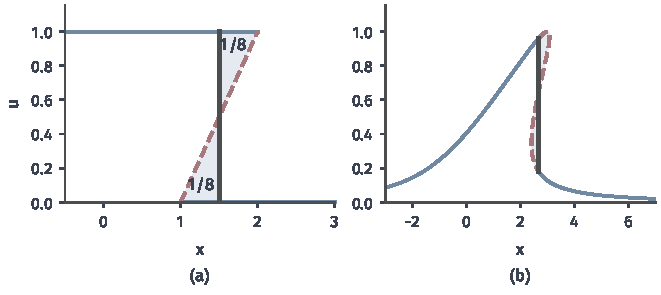
\includegraphics[width=112mm]{figures/06-differential-equations/02-partial-differential-equations/matplotlib/cons-equal-area/figure.pdf}
  \caption{等面积法则。蓝线是单值的解，红色虚线是沿特征线得到的翻转部分，深灰竖线是间断位置，两块浅蓝区域面积相等。(a)斜坡初值在$t=2$，间断位于$x=3/2$，每块面积$1/8$。(b)初值~\eqref{eq:cons-bump}在$t=3$，间断位置由数值积分得到。}
  \label{fig:cons-equal-area}
\end{BookInlineFigure}

贯穿例子~\eqref{eq:cons-bump}的间断路径没有闭式，但可以把上面两条结合起来计算。设$\gamma(t)$是间断位置，$u_\pm$是多值图像在$x=\gamma(t)$处最靠左和最靠右的分支的值，由式~\eqref{eq:cons-burgers-speed}，
\begin{equation}
  \gamma'(t)=\frac{u_-(t)+u_+(t)}{2},\qquad \gamma(T^{*})=\sqrt{3}.
  \label{eq:cons-bump-shock}
\end{equation}

这是一个常微分方程，右端要在每一步解两次特征线方程。数值积分得$\gamma(3)\approx2.677$。图~\ref{fig:cons-bump-shock}(a)中间断从红点长出，特征线不断汇入。(b)显示了波形的演化：间断形成后，峰逐渐被削低，波形的前沿始终保持一个台阶。

\begin{BookInlineFigure}
  \centering
  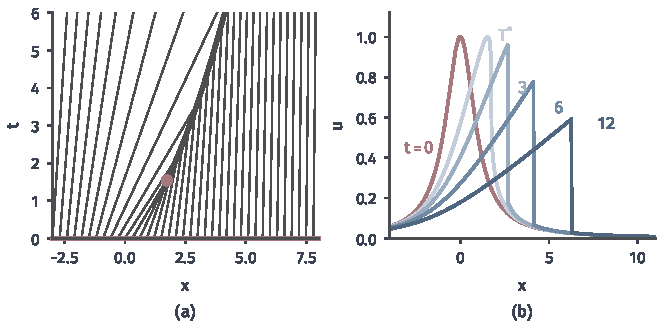
\includegraphics[width=112mm]{figures/06-differential-equations/02-partial-differential-equations/matplotlib/cons-bump-shock/figure.pdf}
  \caption{初值~\eqref{eq:cons-bump}的激波形成之后。(a)细线是特征线，它们都在深灰粗线（数值求解式~\eqref{eq:cons-bump-shock}得到的间断路径）上终止，红点是最早的相交点。(b)红线是$t=0$，蓝色由浅到深是$t=T^{*},3,6,12$，台阶越来越矮。}
  \label{fig:cons-bump-shock}
\end{BookInlineFigure}

\paragraph{同一方程的不同守恒形式}
跳跃条件依赖于哪个量守恒。$C^1$时，Burgers方程乘以$u$，得到同样成立的
\[
  \partial_t\Bigl(\frac{u^2}{2}\Bigr)+\partial_x\Bigl(\frac{u^3}{3}\Bigr)=0 .
\]
两个方程的光滑解完全相同，但把后者看作守恒律时，守恒量是$u^2/2$，通量是$u^3/3$。

对同一组状态$u_-=1$、$u_+=0$，由式~\eqref{eq:cons-shock-speed}，两种写法给出的速度分别是
\[
  s=\frac{1/2-0}{1-0}=\frac12,\qquad
  s=\frac{1/3-0}{1/2-0}=\frac23 .
\]

图~\ref{fig:cons-form-speed}画出这两条路径。所以方程写成哪一种守恒形式不是记号问题，而是在说明哪个量真正守恒；$u\,\partial_xu$这样的非守恒写法在间断处没有定义，也就无从决定速度。

\begin{BookInlineFigure}
  \centering
  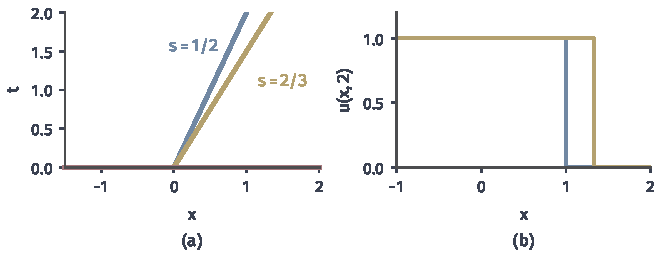
\includegraphics[width=112mm]{figures/06-differential-equations/02-partial-differential-equations/matplotlib/cons-form-speed/figure.pdf}
  \caption{守恒形式决定间断速度，状态$u_-=1$、$u_+=0$。(a)蓝线是以$u$为守恒量得到的路径$s=1/2$，黄线是以$u^2/2$为守恒量得到的路径$s=2/3$。(b)两种情形在$t=2$的形状。}
  \label{fig:cons-form-speed}
\end{BookInlineFigure}

跳跃条件只保证穿过间断的总量收支平衡。$u^{\mathrm{j}}$满足它，$u^{\mathrm{f}}$也满足，所以还要有别的办法检验传播方向是否合理。


\section{熵条件}
\label{sec:cons-entropy}

弱解到底多到什么程度？怎样从中挑出合理的那一个？本节先把多余的解摆出来，再从特征线的方向和小黏性的极限两个角度找到选择规则，最后把规则写成对一切弱解都能检验的不等式。

\paragraph{同一初值的无穷多个弱解}
仍取Burgers方程和阶跃初值$u_0=0$（$x<0$）、$u_0=1$（$x>0$）。上一节的两个解只是一族解的两端。任取$\alpha\in[0,1]$，令
\begin{equation}
  u^{\alpha}(x,t)=\begin{cases}
    0,&x<\alpha t/2,\\
    \alpha,&\alpha t/2<x<\alpha t,\\
    x/t,&\alpha t<x<t,\\
    1,&x\geq t.
  \end{cases}
  \label{eq:cons-weak-family}
\end{equation}

逐块检验。常数块上两个偏导都是零，方程成立；块$u=x/t$上
\[
  \partial_tu+u\,\partial_xu=-\frac{x}{t^2}+\frac{x}{t}\cdot\frac1t=0 .
\]
唯一的跳跃在$x=\alpha t/2$处，两侧是$0$和$\alpha$，由式~\eqref{eq:cons-burgers-speed}，速度应为$\alpha/2$，正好相符。其余两条接缝连续。由定理~\ref{thm:cons-rh}，每个$u^{\alpha}$都是弱解。

图~\ref{fig:cons-weak-family}画出$\alpha=1,\,1/2,\,0$三种情形。$\alpha=1$就是$u^{\mathrm{j}}$，$\alpha=0$就是$u^{\mathrm{f}}$，中间的$\alpha$把一部分扇形换成了向上的跳跃。

\begin{BookInlineFigure}
  \centering
  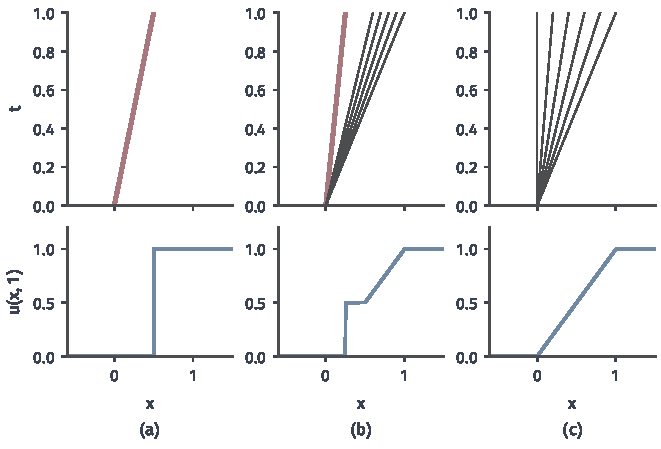
\includegraphics[width=112mm]{figures/06-differential-equations/02-partial-differential-equations/matplotlib/cons-weak-family/figure.pdf}
  \caption{阶跃初值的弱解族~\eqref{eq:cons-weak-family}。上排是$(x,t)$平面，红色粗线是向上的跳跃，细线是扇形中的特征线；下排是$t=1$的形状。(a)$\alpha=1$，全部是跳跃。(b)$\alpha=1/2$，跳跃接扇形。(c)$\alpha=0$，全部是扇形，没有跳跃。}
  \label{fig:cons-weak-family}
\end{BookInlineFigure}

更极端的例子是零初值。任取$b>0$，令
\begin{equation}
  u(x,t)=\begin{cases}
    0,&x<-bt/2,\\
    -b,&-bt/2<x<0,\\
    b,&0<x<bt/2,\\
    0,&x>bt/2.
  \end{cases}
  \label{eq:cons-zero-data}
\end{equation}

三条跳跃线的速度都满足式~\eqref{eq:cons-burgers-speed}：$0$与$-b$之间是$-b/2$，$-b$与$b$之间是$0$，$b$与$0$之间是$b/2$。$t=0$时$u$处处为零，所以这是零初值的非零弱解，见图~\ref{fig:cons-zero-data}。静止的流体从原点自发地向两边散开，总量却分毫不差。所以只算收支账排除不了这样的解。

\begin{BookInlineFigure}
  \centering
  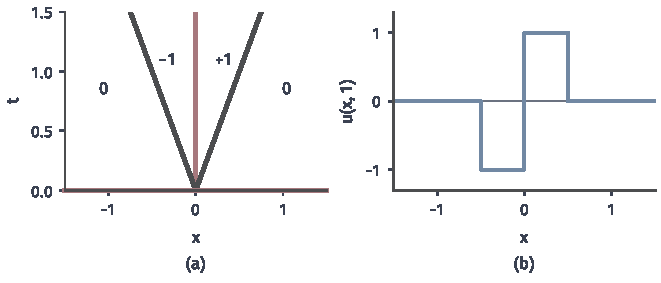
\includegraphics[width=112mm]{figures/06-differential-equations/02-partial-differential-equations/matplotlib/cons-zero-data/figure.pdf}
  \caption{零初值的非零弱解，$b=1$。(a)$(x,t)$平面，数字是各区域的值，红色粗线$x=0$是向上的跳跃，两条深灰粗线是向下的跳跃。(b)$t=1$的形状，正负两块面积相互抵消。}
  \label{fig:cons-zero-data}
\end{BookInlineFigure}

\paragraph{特征线必须汇入间断}
看特征线在间断两侧的走向就能分出好坏。先看图~\ref{fig:cons-lax-in-out}(a)，其中$u_-=1$、$u_+=0$，$s=1/2$。左侧特征线的速度$1$大于$s$，从后面追上间断；右侧特征线的速度$0$小于$s$，被间断追上。两侧的特征线都汇入间断，间断两侧的状态都由更早的初值决定。

(b)中$u_-=0$、$u_+=1$，$s$同样是$1/2$，方向却反了：左侧速度$0$小于$s$，右侧速度$1$大于$s$，特征线都从间断上离开。这些特征线沿途携带的值并不来自初值，只能在间断线上凭空产生。这就是前面的解不唯一的根源：既然这些值无从确定，它们就可以任意选取。

\begin{BookInlineFigure}
  \centering
  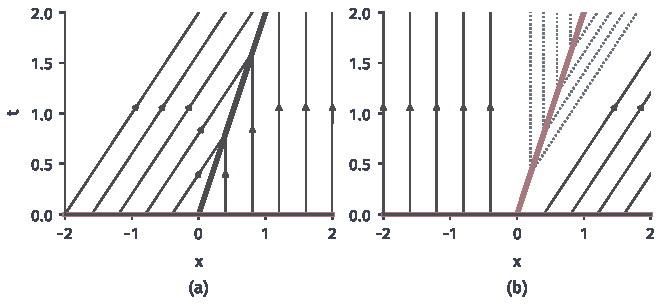
\includegraphics[width=112mm]{figures/06-differential-equations/02-partial-differential-equations/matplotlib/cons-lax-in-out/figure.pdf}
  \caption{两种间断两侧的特征线，$s$都是$1/2$，箭头指向时间增大的方向。(a)$u_-=1$、$u_+=0$（深灰粗线），两侧特征线都汇入。(b)$u_-=0$、$u_+=1$（红色粗线），点线表示从间断上发出的特征线，初值决定不了它们的取值。}
  \label{fig:cons-lax-in-out}
\end{BookInlineFigure}

把这一观察写成条件，就是\term{Lax熵条件}（Lax entropy condition）：
\begin{equation}
  F'(u_-)>s>F'(u_+).
  \label{eq:cons-lax}
\end{equation}

满足这一条件的间断称为\term{激波}（shock wave）。$F$严格凸时条件有更简单的形式。此时$F'$严格递增，$s$是$F'$在$u_-$与$u_+$之间的平均，严格落在两端值之间。所以当$u_-\neq u_+$时，式~\eqref{eq:cons-lax}等价于$F'(u_-)>F'(u_+)$，也就是$u_->u_+$。

对Burgers方程这句话是说，只有向下的跳跃才允许存在。检验前面的例子：$(u_-,u_+)=(1,0)$满足$1>1/2>0$；$(0,1)$要求$0>1/2>1$，不成立。凹的车流通量则相反，要求$u_-<u_+$：前方密度大、后方密度小，正是车辆追上堵车队尾的情形。例如$u_-=0.2$、$u_+=0.8$时
\[
  s=\frac{0.16-0.16}{0.6}=0,\qquad F'(0.2)=0.6>0>-0.6=F'(0.8),
\]
队尾静止不动，两侧的扰动都汇向队尾。

式~\eqref{eq:cons-lax}只适用于分段光滑的解和凸通量。要对一般的有界解下定义，得从这条规则的来源说起。

\paragraph{消失黏性}
真实的流体和车流都有一点扩散：司机会根据前方密度提前调整。在方程里加上小的黏性项，
\begin{equation}
  \partial_tu^{\nu}+\partial_xF(u^{\nu})=\nu\,\partial_{xx}u^{\nu},\qquad \nu>0.
  \label{eq:cons-viscous}
\end{equation}
式~\eqref{eq:cons-viscous}是抛物型方程，第~\ref{chap:diffusion-equations}章的抹平作用使它的解保持光滑，也没有多解的问题。合理的弱解应该是$\nu\to0$时的极限。这种通过\term{消失黏性}（vanishing viscosity）挑选解的做法，可以在Burgers方程上算到底。

寻找行波解$u^{\nu}=U(\xi)$，$\xi=x-st$，$U(\pm\infty)=u_\pm$。代入Burgers方程，得到
\[
  -sU'+UU'=\nu U'' .
\]

对$\xi$积分一次，积分常数记为$C$：
\[
  -sU+\frac{U^2}{2}=\nu U'+C .
\]

令$\xi\to\pm\infty$，$U'\to0$，两端各给一个等式：
\[
  C=-su_-+\frac{u_-^2}{2}=-su_++\frac{u_+^2}{2}.
\]
当$u_-\neq u_+$时，消去$C$得到$s=(u_-+u_+)/2$，Rankine--Hugoniot条件自动出现。把$s$与$C=-u_-u_+/2$代回，一阶方程化为
\begin{equation}
  \nu U'=\frac12(U-u_-)(U-u_+).
  \label{eq:cons-viscous-profile}
\end{equation}

右端在$U$介于$u_-$与$u_+$之间时为负，所以$U$只能沿$\xi$递减。从$\xi=-\infty$的$u_-$走到$\xi=+\infty$的$u_+$，就必须$u_->u_+$。向上的跳跃没有黏性剖面，向下的跳跃才有。解出这个分离变量方程，得到
\begin{equation}
  U(\xi)=\frac{u_-+u_+}{2}-\frac{u_--u_+}{2}\tanh\frac{(u_--u_+)\,\xi}{4\nu}.
  \label{eq:cons-viscous-tanh}
\end{equation}

过渡层的宽度约为$4\nu/(u_--u_+)$，$\nu\to0$时剖面收缩成跳跃，见图~\ref{fig:cons-viscous-profile}。这是黏性对向下跳跃的解释：很薄的一层里，压缩和扩散互相平衡。

\begin{BookInlineFigure}
  \centering
  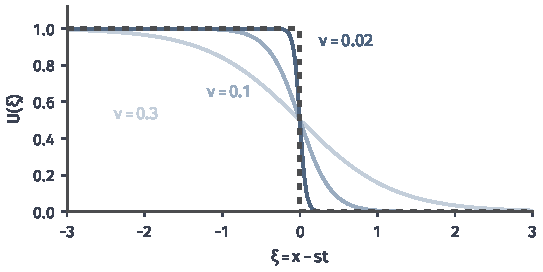
\includegraphics[width=92mm]{figures/06-differential-equations/02-partial-differential-equations/matplotlib/cons-viscous-profile/figure.pdf}
  \caption{Burgers方程的黏性行波~\eqref{eq:cons-viscous-tanh}，$u_-=1$、$u_+=0$。蓝色由浅到深是$\nu=0.3,0.1,0.02$，深灰点线是$\nu\to0$的极限跳跃。}
  \label{fig:cons-viscous-profile}
\end{BookInlineFigure}

向上的阶跃又如何？图~\ref{fig:cons-viscous-fan}把式~\eqref{eq:cons-viscous}从阶跃初值$0$、$1$开始算到$t=1$。数值解没有靠近跳跃$u^{\mathrm{j}}$，而是贴向连续的扇形$u^{\mathrm{f}}$。在弱解族~\eqref{eq:cons-weak-family}中，黏性选中的是$\alpha=0$。

\begin{BookInlineFigure}
  \centering
  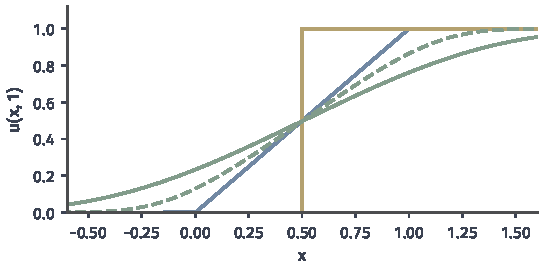
\includegraphics[width=92mm]{figures/06-differential-equations/02-partial-differential-equations/matplotlib/cons-viscous-fan/figure.pdf}
  \caption{阶跃初值$0$、$1$的黏性解在$t=1$的形状，由守恒的显式差分格式算出。绿色实线和虚线是$\nu=0.1$和$\nu=0.02$，蓝线是扇形解$u^{\mathrm{f}}$，黄线是跳跃解$u^{\mathrm{j}}$。$\nu$减小时数值解靠向蓝线。}
  \label{fig:cons-viscous-fan}
\end{BookInlineFigure}

\paragraph{熵不等式}
小黏性留下了什么可以在极限中保存的信息？取任意$C^2$凸函数$\eta$，再取$q$使$q'=\eta'F'$。这样的一对$(\eta,q)$称为\term{熵对}（entropy pair），$\eta$是熵，$q$是\term{熵通量}（entropy flux）。方程~\eqref{eq:cons-viscous}乘以$\eta'(u^{\nu})$，用链式法则整理：
\[
  \partial_t\eta(u^{\nu})+\partial_xq(u^{\nu})
  =\nu\,\partial_{xx}\eta(u^{\nu})-\nu\,\eta''(u^{\nu})\,(\partial_xu^{\nu})^2 .
\]

最后一项因为$\eta$凸而非正，它记录了扩散带来的耗散，正是这一项在极限中留下了方向。乘以$\varphi\geq0$并积分，分部积分后丢掉非负的耗散项，得到
\[
  \iint\bigl(\eta(u^{\nu})\,\partial_t\varphi+q(u^{\nu})\,\partial_x\varphi\bigr)\,\mathrm{d}x\,\mathrm{d}t
  \geq-\nu\iint\eta(u^{\nu})\,\partial_{xx}\varphi\,\mathrm{d}x\,\mathrm{d}t .
\]
假定$u^{\nu}$一致有界且几乎处处收敛，令$\nu\to0$，右端趋于零，留下一个不含$\nu$的不等式。这段推导只说明了不等式的来源，下面把它取作定义。

\begin{definition}[熵解]
\label{def:cons-entropy-solution}
设$F\in C^1(\mathbb{R})$，$u_0\in L^{\infty}(\mathbb{R})$。函数$u\in L^{\infty}(\mathbb{R}\times(0,\infty))$称为问题~\eqref{eq:cons-law}、\eqref{eq:cons-initial}的\term{熵解}（entropy solution），若对每个$C^2$凸函数$\eta$、满足$q'=\eta'F'$的$q$，以及每个非负的$\varphi\in C_c^{\infty}(\mathbb{R}\times(0,\infty))$，
\begin{equation}
  \int_0^{\infty}\!\!\int_{\mathbb{R}}\bigl(\eta(u)\,\partial_t\varphi+q(u)\,\partial_x\varphi\bigr)\,\mathrm{d}x\,\mathrm{d}t\geq0 ,
  \label{eq:cons-entropy-ineq}
\end{equation}
并且对每个$R>0$，初值在下述意义下取到：
\begin{equation}
  \operatorname*{ess\,lim}_{t\downarrow0}\int_{-R}^{R}\lvert u(x,t)-u_0(x)\rvert\,\mathrm{d}x=0 .
  \label{eq:cons-entropy-initial}
\end{equation}
\end{definition}

不等式~\eqref{eq:cons-entropy-ineq}是$\partial_t\eta(u)+\partial_xq(u)\leq0$的弱形式。取$\eta(u)=u$、$q=F$和$\eta(u)=-u$、$q=-F$，两者都是凸的，两个不等式合起来给出等式，再结合式~\eqref{eq:cons-entropy-initial}，熵解一定是弱解。$C^1$解由链式法则使式~\eqref{eq:cons-entropy-ineq}取等号，所以经典解也是熵解。

“熵”的名字来自气体动力学，那里的物理熵经过激波只增不减；数学上取凸函数，符号相反，所以$\eta$的总量只减不增。凸性的作用是把扩散耗散的符号固定下来。可以把$\eta(u)$想成一种能量：光滑时它和$u$一样守恒，只在间断处被消耗。

\paragraph{跨间断的熵不等式}
分段光滑的解要满足什么条件？重复定理~\ref{thm:cons-rh}的散度计算，把$(u,F(u))$换成$(\eta(u),q(u))$。在间断线两侧光滑部分的贡献为零，只留下线积分，于是式~\eqref{eq:cons-entropy-ineq}等价于
\begin{equation}
  q(u_+)-q(u_-)-s\bigl(\eta(u_+)-\eta(u_-)\bigr)\leq0 .
  \label{eq:cons-jump-entropy}
\end{equation}

左端是单位时间内在间断上产生的熵。取Burgers方程、$\eta=u^2/2$、$q=u^3/3$，并用$s=(u_-+u_+)/2$。记$\Delta=u_+-u_-$，直接展开：
\[
  \begin{aligned}
    \frac{u_+^3-u_-^3}{3}-\frac{(u_-+u_+)(u_+^2-u_-^2)}{4}
    &=\Delta\,\frac{4(u_+^2+u_+u_-+u_-^2)-3(u_-+u_+)^2}{12}\\
    &=\frac{\Delta^3}{12}.
  \end{aligned}
\]

所以间断上的能量变化率恰好是
\begin{equation}
  \frac{(u_+-u_-)^3}{12},
  \label{eq:cons-energy-rate}
\end{equation}
它非正当且仅当$u_+\leq u_-$。向下的跳跃消耗能量，向上的跳跃产生能量。

用斜坡解~\eqref{eq:cons-ramp-shock}核对一下。$t\geq1$时，在包含间断的大区间上，$\int u^2/2\,\mathrm{d}x$的增长率是$1/4$，因为$u=1$的区域以速度$1/2$延伸，每单位长度带能量$1/2$。左端流入能量的速率是$q(1)=1/3$。两者相差
\[
  \frac13-\frac14=\frac{1}{12},
\]
正是式~\eqref{eq:cons-energy-rate}在$(u_-,u_+)=(1,0)$时给出的耗散率。

零初值的解~\eqref{eq:cons-zero-data}同样可以算账。中间的跳跃$-b\to b$产生能量$(2b)^3/12=2b^3/3$，两侧的跳跃各消耗$b^3/12$，净产生率为$b^3/2$，这正是总能量$b^3t/2$的增长率。这个解违反熵不等式，错就错在中间那条向上的跳跃。

图~\ref{fig:cons-energy-decay}显示贯穿例子的情况：$T^{*}$之前能量守恒，激波形成之后能量按式~\eqref{eq:cons-energy-rate}减少，而总量一直不变。这是守恒律与熵的区别：总量是真正守恒的量，熵只有在光滑时才守恒。

\begin{BookInlineFigure}
  \centering
  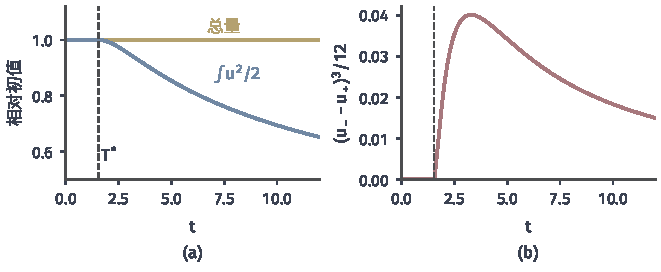
\includegraphics[width=112mm]{figures/06-differential-equations/02-partial-differential-equations/matplotlib/cons-energy-decay/figure.pdf}
  \caption{初值~\eqref{eq:cons-bump}的总量与能量。(a)黄线是总量$\int u\,\mathrm{d}x$相对初值的比，蓝线是能量$\int u^2/2\,\mathrm{d}x$相对初值的比，虚线是$T^{*}$。(b)激波上的耗散率$(u_--u_+)^3/12$，$T^{*}$之前为零。}
  \label{fig:cons-energy-decay}
\end{BookInlineFigure}

\paragraph{一族就够：Kruzhkov熵}
定义要求对所有凸熵成立，用起来需要一族足够简单的代表。对每个$k\in\mathbb{R}$，令
\begin{equation}
  \eta_k(u)=\lvert u-k\rvert,\qquad q_k(u)=\operatorname{sgn}(u-k)\bigl(F(u)-F(k)\bigr),
  \label{eq:cons-kruzhkov-pair}
\end{equation}
这称为\term{Kruzhkov熵}（Kruzhkov entropy）。它不是$C^2$的，但下面的引理说明，只需检验这一族。

\begin{lemma}[Kruzhkov熵的充分性]
\label{lem:cons-kruzhkov}
设$F\in C^1$，$u$有界。式~\eqref{eq:cons-entropy-ineq}对所有$C^2$凸熵对成立，当且仅当对每个$k\in\mathbb{R}$和每个$\varphi\geq0$，
\begin{equation}
  \int_0^{\infty}\!\!\int_{\mathbb{R}}\bigl(\lvert u-k\rvert\,\partial_t\varphi+q_k(u)\,\partial_x\varphi\bigr)\,\mathrm{d}x\,\mathrm{d}t\geq0 .
  \label{eq:cons-kruzhkov}
\end{equation}
\end{lemma}

\begin{proof}
必要性：取$C^2$凸函数及与之配对的熵通量
\[
  \eta_\delta(u)=\sqrt{(u-k)^2+\delta^2}-\delta,\qquad
  q_\delta(u)=\int_k^u\eta_\delta'(w)F'(w)\,\mathrm{d}w .
\]
$\delta\to0$时，在有界集上$\eta_\delta\to\lvert u-k\rvert$，$q_\delta\to q_k$，且都是一致收敛，不等式取极限成立。

充分性：记$\lVert u\rVert_{L^\infty}\leq M$。对$C^2$凸函数$\eta$，在$[-M,M]$上有表示
\[
  \eta(u)=\alpha u+\beta+\frac12\int_{-M}^{M}\eta''(k)\,\lvert u-k\rvert\,\mathrm{d}k .
\]
这是因为两端的二阶导数都是$\eta''$，差是仿射函数。

对上式求导，得到
\[
  \eta'(u)=\alpha+\frac12\int_{-M}^{M}\eta''(k)\operatorname{sgn}(u-k)\,\mathrm{d}k .
\]

乘以$F'(u)$再积分，熵通量有对应的表示：
\[
  q(u)=\alpha F(u)+\beta'+\frac12\int_{-M}^{M}\eta''(k)\,q_k(u)\,\mathrm{d}k .
\]

取$k=M$和$k=-M$，式~\eqref{eq:cons-kruzhkov}中$\lvert u-k\rvert$分别是$M-u$和$u+M$，两个不等式合起来说明$u$满足式~\eqref{eq:cons-rh-weak}形式的等式，于是仿射部分的贡献为零。常数项$\beta,\beta'$积分后也为零。其余部分是式~\eqref{eq:cons-kruzhkov}按非负权重$\eta''(k)/2$对$k$的积分，所以非负。
\end{proof}

现在可以回答跨间断的问题：对一个满足跳跃条件的间断，熵条件到底要求什么。记$L(k)$是通量图像上连接两个状态的弦，
\begin{equation}
  L(k)=F(u_-)+s\,(k-u_-).
  \label{eq:cons-chord}
\end{equation}

\begin{theorem}[跨间断的熵判据]
\label{thm:cons-chord}
设$F\in C^1$，$u_-\neq u_+$，$s$由式~\eqref{eq:cons-shock-speed}给出。则式~\eqref{eq:cons-jump-entropy}对所有$C^2$凸熵对成立，当且仅当对$u_-$与$u_+$之间的每个$k$，
\begin{equation}
  \begin{cases}
    F(k)\leq L(k),&u_->u_+,\\
    F(k)\geq L(k),&u_-<u_+.
  \end{cases}
  \label{eq:cons-oleinik}
\end{equation}
特别地，$F$严格凸时，熵判据等价于$u_->u_+$，也等价于式~\eqref{eq:cons-lax}。
\end{theorem}

\begin{proof}
记$D(\eta,q)$是式~\eqref{eq:cons-jump-entropy}的左端。$D$关于$(\eta,q)$是线性的，由引理~\ref{lem:cons-kruzhkov}中的表示，只需计算$D_k=D(\eta_k,q_k)$。仿射部分贡献$\alpha(F(u_+)-F(u_-)-s(u_+-u_-))=0$，这用到了跳跃条件。

$k$不在$u_-$与$u_+$之间时，$\operatorname{sgn}(u-k)$在两个状态上相同，$D_k$是跳跃条件的一个倍数，等于零。

设$u_->k>u_+$。此时$\eta_k(u_-)=u_--k$，$\eta_k(u_+)=k-u_+$，相应的熵通量是$F(u_-)-F(k)$和$F(k)-F(u_+)$。代入得到
\[
  D_k=2F(k)-F(u_+)-F(u_-)-s\,(2k-u_+-u_-).
\]

由式~\eqref{eq:cons-chord}和跳跃条件$F(u_+)=F(u_-)+s(u_+-u_-)$，上式整理为
\[
  D_k=2\bigl(F(k)-L(k)\bigr).
\]
所以$D_k\leq0$当且仅当$F(k)\leq L(k)$。$u_-<k<u_+$时两个符号都反过来，$D_k=-2(F(k)-L(k))$，于是$D_k\leq0$当且仅当$F(k)\geq L(k)$。

必要性取$D_k\leq0$对$C^2$逼近的极限；充分性把$D_k\leq0$按非负权重$\eta''(k)/2$积分。

$F$严格凸时，弦严格在图像上方，$F(k)<L(k)$，第二种情形不可能，第一种情形总成立。
\end{proof}

式~\eqref{eq:cons-oleinik}称为\term{Oleinik条件}（Oleinik condition），图~\ref{fig:cons-oleinik-chord}是它的几何图景。它同时覆盖凸与非凸通量，比式~\eqref{eq:cons-lax}更一般：跳跃能否存在，取决于通量图像在两个状态之间落在弦的哪一边。用$k=1/2$检验$(u_-,u_+)=(1,0)$：$F(1/2)=1/8$，$L(1/2)=1/4$，$D_k=2(1/8-1/4)=-1/4\leq0$，熵不等式成立。

\begin{BookInlineFigure}
  \centering
  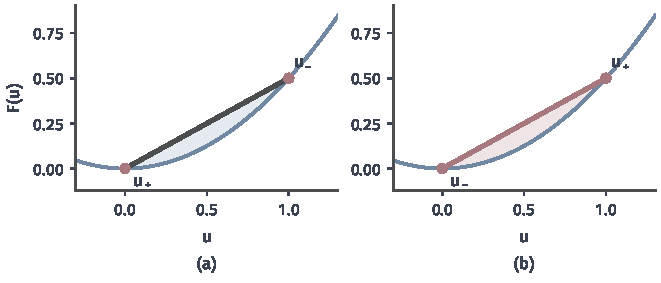
\includegraphics[width=112mm]{figures/06-differential-equations/02-partial-differential-equations/matplotlib/cons-oleinik-chord/figure.pdf}
  \caption{Oleinik条件，$F=u^2/2$（蓝）。两图的弦相同，红点是两个状态。(a)$u_->u_+$，要求图像在弦下方（浅蓝），成立。(b)$u_-<u_+$，要求图像在弦上方，凸函数的图像却在下方（浅红），不成立。}
  \label{fig:cons-oleinik-chord}
\end{BookInlineFigure}

消失黏性的说明到这里还只是形式推导。严格的结论是：$F\in C^1$、$u_0\in L^{\infty}$时，式~\eqref{eq:cons-viscous}的解在$\nu\to0$时在$L^1_{\mathrm{loc}}$中收敛到熵解。证明需要用到解的一致有界性、全变差估计和紧性论证，篇幅较长，读者可查阅Kruzhkov于1970年发表的原始论文或双曲守恒律的专著。这个定理说明熵条件的选择与物理上的小黏性是一致的。


\section{Riemann问题}
\label{sec:cons-riemann}

最简单的不连续初值是左右两个常状态：
\begin{equation}
  u_0(x)=\begin{cases}u_l,&x<0,\\u_r,&x>0.\end{cases}
  \label{eq:cons-riemann-data}
\end{equation}
这称为\term{Riemann问题}（Riemann problem）。守恒、特征线和熵条件在这里都能落实成手算。

有一条结构可以先用上。方程和初值在缩放$(x,t)\mapsto(\lambda x,\lambda t)$下不变，若解唯一（下一节证明），解就只依赖于比值$\xi=x/t$，形如$u=w(\xi)$。这样的解称为\term{自相似解}（self-similar solution）。在$(x,t)$平面上，它沿着从原点出发的每条射线取常值。

本节先设$F$严格凸。此时$F'$严格递增，按上一节的结论，$u_l>u_r$时阶跃本身是可接受的间断，$u_l<u_r$时不是。这两种情形分别对应两种完全不同的波。

\subsection{激波}
\label{subsec:cons-shock}

左状态大于右状态时，$F'(u_l)>F'(u_r)$，左边的特征线比右边的快，迎面相撞，只能产生间断。

\begin{theorem}[激波解]
\label{thm:cons-shock}
设$F\in C^1$严格凸，$u_l>u_r$。令
\begin{equation}
  s=\frac{F(u_l)-F(u_r)}{u_l-u_r},\qquad
  u(x,t)=\begin{cases}u_l,&x<st,\\u_r,&x>st.\end{cases}
  \label{eq:cons-shock-solution}
\end{equation}
则$u$是Riemann问题的熵解。
\end{theorem}

\begin{proof}
$u$分块为常数，满足方程。$s$由式~\eqref{eq:cons-shock-speed}给出，跳跃条件成立。由定理~\ref{thm:cons-chord}，$u_->u_+$时式~\eqref{eq:cons-jump-entropy}对所有凸熵对成立，所以式~\eqref{eq:cons-entropy-ineq}成立。最后，$u$与初值只在宽度为$\lvert s\rvert t$的区间上不同，差不超过$u_l-u_r$，式~\eqref{eq:cons-entropy-initial}成立。
\end{proof}

波速由两侧状态共同决定，任何一侧单独都定不下来。表~\ref{tab:cons-shock-examples}列出几组数据。Burgers方程的波速是两侧状态的算术平均，这是平方通量的特殊之处；最后一行的通量$F=u^4/4$严格凸，波速$15/4$并不等于两侧传播速度的平均$9/2$。每一行都满足$F'(u_l)>s>F'(u_r)$。

\begin{BookInlineTable}
  \centering
  \caption{激波速度的手算。前四行是Burgers方程，第五行$F=u^4/4$，每一行都验证了$F'(u_l)>s>F'(u_r)$。}
  \label{tab:cons-shock-examples}
  \begin{tabular}{cccccc}
    \toprule
    通量 & $u_l$ & $u_r$ & $s$ & $F'(u_l)$ & $F'(u_r)$\\
    \midrule
    $u^2/2$ & $2$ & $0$ & $1$ & $2$ & $0$\\
    $u^2/2$ & $2$ & $1$ & $3/2$ & $2$ & $1$\\
    $u^2/2$ & $1$ & $-1$ & $0$ & $1$ & $-1$\\
    $u^2/2$ & $0$ & $-2$ & $-1$ & $0$ & $-2$\\
    $u^4/4$ & $2$ & $1$ & $15/4$ & $8$ & $1$\\
    \bottomrule
  \end{tabular}
\end{BookInlineTable}

取第一行$u_l=2$、$u_r=0$，$s=1$，解在图~\ref{fig:cons-riemann-shock}中。用矩形$[-1,3]\times[0,1]$核对收支：初始总量是$2\cdot1=2$，$t=1$时$x<1$的部分长度为$2$，总量是$4$，左端流入$F(2)\cdot1=2$，右端流出$0$，正好$2+2=4$。第三行的$s=0$说明波速可以为零，第四行的$s=-1$说明激波可以向左传播。

\begin{BookInlineFigure}
  \centering
  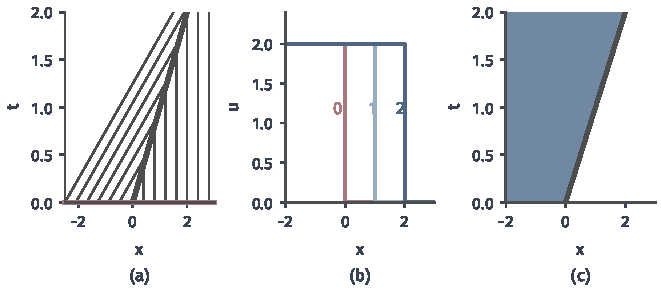
\includegraphics[width=112mm]{figures/06-differential-equations/02-partial-differential-equations/matplotlib/cons-riemann-shock/figure.pdf}
  \caption{Burgers方程的Riemann问题$u_l=2$、$u_r=0$，$s=1$。(a)特征线（细线）从两侧汇入激波（深灰粗线）。(b)红线是$t=0$，蓝色由浅到深是$t=1,2$。(c)时空平面上的场，颜色越深值越大。}
  \label{fig:cons-riemann-shock}
\end{BookInlineFigure}

\subsection{稀疏波}
\label{subsec:cons-rarefaction}

左状态小于右状态时，$F'(u_l)<F'(u_r)$，左边的特征线比右边的慢，它们彼此分开。图~\ref{fig:cons-riemann-fan}(a)中，浅红的楔形区域没有任何特征线到达，式~\eqref{eq:cons-implicit}在那里什么也没有告诉我们。阶跃本身还是可以当作弱解，但它在上一节已经被熵条件排除，楔形必须用别的东西填满。

\begin{BookInlineFigure}
  \centering
  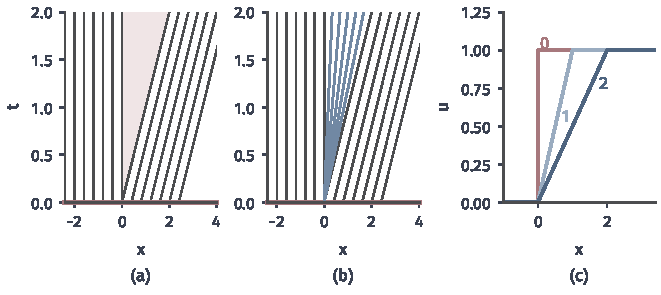
\includegraphics[width=112mm]{figures/06-differential-equations/02-partial-differential-equations/matplotlib/cons-riemann-fan/figure.pdf}
  \caption{Burgers方程的Riemann问题$u_l=0$、$u_r=1$。(a)只画初始线出发的特征线，留下一片浅红的空白楔形。(b)从原点发出的扇形特征线（蓝）填满楔形。(c)红线是$t=0$，蓝色由浅到深是$t=1,2$，斜坡的宽度随时间线性增长。}
  \label{fig:cons-riemann-fan}
\end{BookInlineFigure}

用自相似的形式求解。把$u=w(\xi)$，$\xi=x/t$代入式~\eqref{eq:cons-quasilinear}，$\partial_tu=-\xi w'/t$，$\partial_xu=w'/t$，得到
\[
  \frac{w'(\xi)}{t}\bigl(F'(w(\xi))-\xi\bigr)=0 .
\]

所以每一点要么$w'=0$（常状态），要么$F'(w(\xi))=\xi$。后者说明，填补楔形的解满足$F'(w)=\xi$，也就是把初始间断点看成同时发出所有速度的特征线的源头：每条射线$x=\xi t$就是一条特征线，速度恰好是$\xi$。这样得到的解称为\term{稀疏波}（rarefaction wave）。

\begin{theorem}[稀疏波解]
\label{thm:cons-rarefaction}
设$F\in C^2$，在$[u_l,u_r]$上$F''>0$，$u_l<u_r$。令
\begin{equation}
  u(x,t)=\begin{cases}
    u_l,&x\leq F'(u_l)\,t,\\
    (F')^{-1}(x/t),&F'(u_l)\,t<x<F'(u_r)\,t,\\
    u_r,&x\geq F'(u_r)\,t.
  \end{cases}
  \label{eq:cons-rarefaction}
\end{equation}
则$u$连续（$t>0$），并且是Riemann问题的熵解。
\end{theorem}

\begin{proof}
$F'$在$[u_l,u_r]$上严格递增，逆函数$(F')^{-1}$是$C^1$的，所以式~\eqref{eq:cons-rarefaction}有定义。在扇形边界上它的值分别是$u_l$、$u_r$，$u$在$t>0$连续。

在扇形内，记$w=(F')^{-1}$，有$F''(w)\,w'=1$，于是
\[
  \partial_tu+F'(u)\,\partial_xu
  =-\frac{x}{t^2}w'+\frac{x}{t}\cdot\frac{w'}{t}=0 .
\]

$u$在各块上是$C^1$的，满足方程，由链式法则，每一块上$\partial_t\eta(u)+\partial_xq(u)=0$。两条接缝上$u$连续，式~\eqref{eq:cons-jump-entropy}的左端为零。所以式~\eqref{eq:cons-entropy-ineq}取等号成立。最后，$u$只在宽度不超过$\max\lvert F'\rvert\,t$的区间上与初值不同，差不超过$u_r-u_l$，式~\eqref{eq:cons-entropy-initial}成立。
\end{proof}

Burgers方程$F'(u)=u$，$(F')^{-1}$是恒等映射，取$(u_l,u_r)=(0,1)$，得到
\begin{equation}
  u(x,t)=\frac{x}{t},\qquad 0<x<t,
  \label{eq:cons-burgers-fan}
\end{equation}
这正是前面的$u^{\mathrm{f}}$。$F=u^4/4$、$(u_l,u_r)=(1,2)$时，$F'(u)=u^3$，扇形占据$1<x/t<8$，解是$u=(x/t)^{1/3}$。扇形边缘的速度由两侧状态各自决定，而不是取什么平均：左边缘$F'(u_l)$，右边缘$F'(u_r)$。

\paragraph{扇形是连续依赖的结果}
稀疏波可以由经典解的极限得到。把阶跃$0$、$1$替换成宽度为$\varepsilon$的斜坡，$u_0=x/\varepsilon$（$0\leq x\leq\varepsilon$）。这个初值单调不减，定理~\ref{thm:cons-lifespan}说解永远不会失去光滑性。由特征线$x=x_0+(x_0/\varepsilon)t$反解$x_0=\varepsilon x/(\varepsilon+t)$，得到
\begin{equation}
  u^{\varepsilon}(x,t)=\frac{x}{\varepsilon+t},\qquad 0\leq x\leq\varepsilon+t .
  \label{eq:cons-smoothed-step}
\end{equation}

令$\varepsilon\to0$，式~\eqref{eq:cons-smoothed-step}收敛到扇形~\eqref{eq:cons-burgers-fan}，如图~\ref{fig:cons-smoothed-step}。所以向上的阶跃是一个不稳定的状态：无论把初值磨得多么轻微，解都立刻选择扇形。跳跃解$u^{\mathrm{j}}$经不起这样的扰动，这是排除它的又一条理由。

\begin{BookInlineFigure}
  \centering
  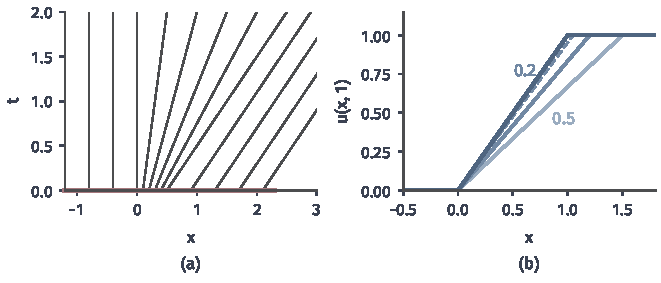
\includegraphics[width=112mm]{figures/06-differential-equations/02-partial-differential-equations/matplotlib/cons-smoothed-step/figure.pdf}
  \caption{磨光的阶跃。(a)$\varepsilon=0.5$的特征线，从斜坡出发的特征线彼此张开，永不相交。(b)解~\eqref{eq:cons-smoothed-step}在$t=1$的形状，蓝色由浅到深是$\varepsilon=0.5,0.2$，虚线是$\varepsilon=0.05$，最深的蓝线是扇形。}
  \label{fig:cons-smoothed-step}
\end{BookInlineFigure}

表~\ref{tab:cons-wave-comparison}把三种候选放在一起对比。

\begin{BookInlineTable}
  \centering
  \caption{严格凸通量下的三种波。}
  \label{tab:cons-wave-comparison}
  \begin{tabular}{cccc}
    \toprule
    & 激波 & 稀疏波 & 扩张间断\\
    \midrule
    状态 & $u_l>u_r$ & $u_l<u_r$ & $u_l<u_r$\\
    连续性 & 跳跃 & 连续 & 跳跃\\
    特征线 & 汇入 & 张开并填满 & 从间断发出\\
    能量（Burgers） & 减少 & 守恒 & 增加\\
    熵条件 & 满足 & 满足 & 违反\\
    \bottomrule
  \end{tabular}
\end{BookInlineTable}

\paragraph{波的相遇：方波}
Riemann解可以拼起来，用来算一般的初值。取Burgers方程和方波
\[
  u_0(x)=\begin{cases}1,&0<x<1,\\0,&\text{其他}.\end{cases}
\]

$x=0$处是向上的阶跃，产生扇形$u=x/t$；$x=1$处是向下的阶跃，产生激波，速度$1/2$。所以$t\leq2$时
\[
  u(x,t)=\begin{cases}x/t,&0<x<t,\\1,&t<x<1+t/2,\\0,&\text{其他}.\end{cases}
\]

扇形的右边缘$x=t$追赶激波$x=1+t/2$，相遇于$t=2$、$x=2$。此后激波左侧的状态不再是常数，而是扇形的值$\gamma/t$，右侧仍是$0$。由式~\eqref{eq:cons-burgers-speed}，激波位置$\gamma(t)$满足
\[
  \gamma'(t)=\frac{\gamma(t)}{2t},\qquad \gamma(2)=2 .
\]

分离变量解得$\gamma(t)=\sqrt{2t}$。于是$t\geq2$时的解是
\begin{equation}
  u(x,t)=\begin{cases}x/t,&0<x<\sqrt{2t},\\0,&\text{其他}.\end{cases}
  \label{eq:cons-box-late}
\end{equation}

波形成为一个三角形，高度$\gamma/t=\sqrt{2/t}$按$t^{-1/2}$衰减，底宽$\sqrt{2t}$按$t^{1/2}$增长。面积是
\[
  \frac12\cdot\sqrt{2t}\cdot\sqrt{\frac2t}=1 ,
\]
与初值的总量一致。图~\ref{fig:cons-box-interaction}展示了这个过程。

\begin{BookInlineFigure}
  \centering
  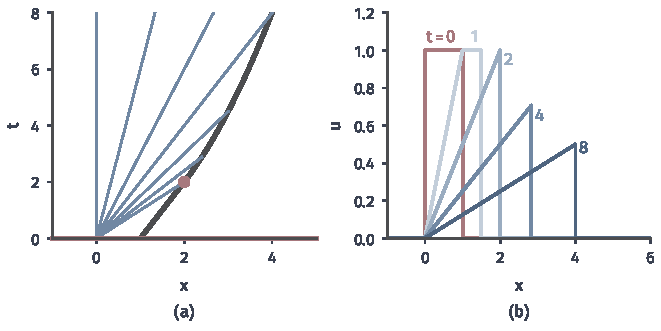
\includegraphics[width=112mm]{figures/06-differential-equations/02-partial-differential-equations/matplotlib/cons-box-interaction/figure.pdf}
  \caption{方波的演化。(a)蓝线是从原点发出的扇形特征线，深灰粗线是激波，红点$(2,2)$是扇形右边缘追上激波的位置，此后激波沿$x=\sqrt{2t}$弯曲。(b)红线是$t=0$，蓝色由浅到深是$t=1,2,4,8$，方波先变成梯形，再变成衰减的三角形。}
  \label{fig:cons-box-interaction}
\end{BookInlineFigure}

\paragraph{更一般的通量}
通量不凸时，单一的激波或扇形可能都不行，解由两者复合而成。规律是：$u_l>u_r$时取$F$在$[u_r,u_l]$上的上凹包络，$u_l<u_r$时取下凸包络；包络的直线段对应间断，严格弯曲的部分对应扇形。这一构造的完整证明要逐段验证Oleinik条件，较为繁琐，读者可查阅双曲守恒律的专著。下面验证一个具体的例子。

取$F(u)=u^3/3$，$(u_l,u_r)=(1,-1)$。$F$在$u<0$时凹，$u>0$时凸。从$(1,1/3)$作切线，切$F$的图像于$a<0$，条件是切线斜率等于弦斜率：
\[
  a^2=\frac{1/3-a^3/3}{1-a}=\frac{1+a+a^2}{3}.
\]

整理得$2a^2-a-1=0$，舍去$a=1$，取$a=-1/2$。于是解由三段组成：从$1$跳到$-1/2$的激波，速度$s=a^2=1/4$；然后是由$w^2=\xi$定出的扇形，$w=-\sqrt{\xi}$，$1/4<\xi<1$；最后是常状态$-1$。

检验激波部分。由式~\eqref{eq:cons-chord}，弦是$L(k)=1/3+(k-1)/4$，于是
\[
  F(k)-L(k)=\frac{4k^3-3k-1}{12}=\frac{(k-1)(2k+1)^2}{12}.
\]
在$k\in[-1/2,1]$上这个量非正，式~\eqref{eq:cons-oleinik}成立。切点$k=-1/2$处恰好为零，这正是激波与扇形相接的位置。

图~\ref{fig:cons-cubic-compound}把这个解和一个迎风差分格式的数值解画在一起，两者吻合。这种复合波说明，严格凸通量下的二分法不能照搬到一般通量。

\begin{BookInlineFigure}
  \centering
  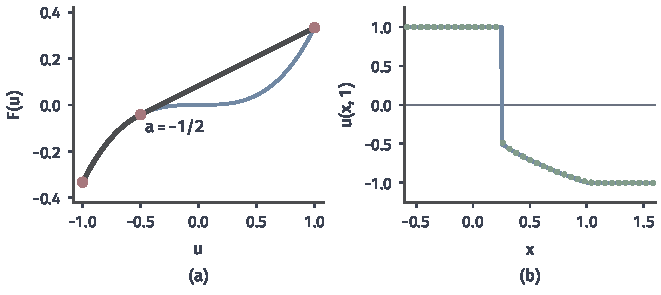
\includegraphics[width=112mm]{figures/06-differential-equations/02-partial-differential-equations/matplotlib/cons-cubic-compound/figure.pdf}
  \caption{非凸通量$F=u^3/3$的Riemann问题$u_l=1$、$u_r=-1$。(a)蓝线是$F$，深灰粗线是上凹包络，红点是端点和切点$a=-1/2$。(b)蓝线是$t=1$的精确解（激波接扇形），绿点是空间步长$2\times10^{-3}$的迎风格式的数值解。}
  \label{fig:cons-cubic-compound}
\end{BookInlineFigure}


\section{唯一性与稳定性}
\label{sec:cons-uniqueness}

熵条件排除了前面所有的反例，但这并不等于只剩下一个解。怎样证明同一初值的熵解只有一个？办法是比较两个熵解：证明它们的积分距离不会随时间增大。

\paragraph{距离为什么不增}
先看一个算得出的例子。比较斜坡初值~\eqref{eq:cons-ramp}的解$u$和阶跃初值的解$v$，阶跃位于$x=1/2$，左$1$右$0$。$v$是激波解，位置$x=(1+t)/2$。$u$在$t<1$时由式~\eqref{eq:cons-ramp-solution}给出，$t\geq1$时由式~\eqref{eq:cons-ramp-shock}给出。

$t<1$时，两个解只在区间$(t,1)$上不同。在激波位置$x=(1+t)/2$处，$u$的值是$1/2$，所以差的图像是两个全等的三角形，底为$(1-t)/2$，高为$1/2$。于是
\begin{equation}
  \lVert u(\cdot,t)-v(\cdot,t)\rVert_1=\frac{1-t}{4},\qquad 0\leq t\leq1.
  \label{eq:cons-merge-distance}
\end{equation}

$t=1$时距离为零，此后两个解完全相同，见图~\ref{fig:cons-merge-l1}。距离在减小，而且激波吞掉了两个初值之间的差别。

\begin{BookInlineFigure}
  \centering
  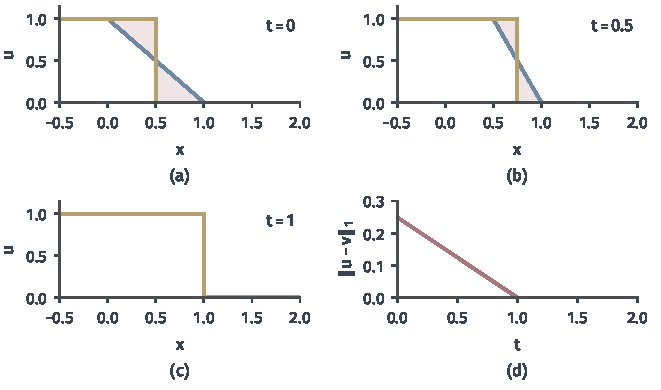
\includegraphics[width=112mm]{figures/06-differential-equations/02-partial-differential-equations/matplotlib/cons-merge-l1/figure.pdf}
  \caption{两个熵解的距离。蓝线是斜坡初值的解，黄线是阶跃初值的解，浅红区域的面积是两者的$L^1$距离。(a)$t=0$。(b)$t=0.5$。(c)$t=1$，两个解重合。(d)距离随时间的变化，$t\leq1$时为$(1-t)/4$，此后为零。}
  \label{fig:cons-merge-l1}
\end{BookInlineFigure}

\paragraph{收缩定理}
一般情形的结论如下。式中的常数$L$是系统中最大的传播速度，它决定了外部区域的影响能传多快。

\begin{theorem}[局部$L^1$收缩]
\label{thm:cons-contraction}
设$F\in C^1(\mathbb{R})$，$u,v$是初值$u_0,v_0\in L^{\infty}(\mathbb{R})$的两个熵解。取$M$使$\lvert u\rvert,\lvert v\rvert\leq M$几乎处处成立，令$L=\max_{\lvert w\rvert\leq M}\lvert F'(w)\rvert$。则对每个$R>0$和几乎处处的$T>0$，
\begin{equation}
  \int_{-R}^{R}\lvert u(x,T)-v(x,T)\rvert\,\mathrm{d}x
  \leq\int_{-R-LT}^{R+LT}\lvert u_0(x)-v_0(x)\rvert\,\mathrm{d}x .
  \label{eq:cons-local-contraction}
\end{equation}
\end{theorem}

图~\ref{fig:cons-cone}是这个不等式的几何含义。$t=T$时区间$[-R,R]$上的差，只由底边$[-R-LT,R+LT]$上的初值差决定，侧边以速度$L$向内收缩。间断可以穿过这个梯形，账依然成立。

\begin{BookInlineFigure}
  \centering
  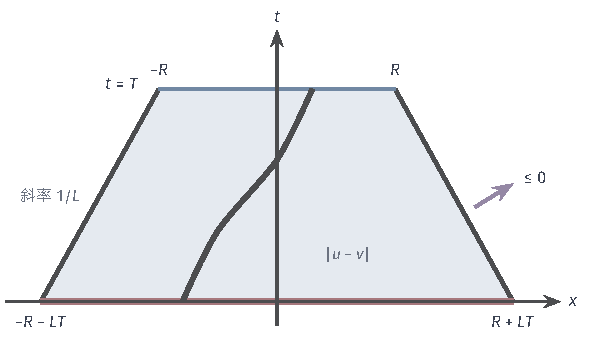
\includegraphics[width=99.8mm]{figures/06-differential-equations/02-partial-differential-equations/tikz/cons-cone/figure.pdf}
  \caption{依赖域梯形。底边（红）是初值差的积分范围，顶边（蓝）是$t=T$时的积分范围，两条侧边（深灰）的速度为$L$。紫色箭头表示穿过侧边的净流量不为正，即差不会从侧边流入。梯形内的深灰曲线是一条可能的间断线。}
  \label{fig:cons-cone}
\end{BookInlineFigure}

证明的难处在于$u$和$v$都不光滑，不能直接相减再求导。若是光滑解，$w=u-v$满足线性输运方程，$\lvert w\rvert$沿特征线的积分不增，结论立刻得到。Kruzhkov的办法是\term{变量加倍}（doubling of variables）：让$u$依赖$(x,t)$，$v$依赖独立的$(y,s)$，在式~\eqref{eq:cons-kruzhkov}中用一个解的值充当另一个解的常数$k$，最后用很窄的权重把$(y,s)$压回$(x,t)$，如图~\ref{fig:cons-doubling}。常数$k$在这里扮演的角色正是Kruzhkov熵的用处：熵不等式对每个$k$成立，$k$就可以取另一个解的值。

\begin{BookInlineFigure}
  \centering
  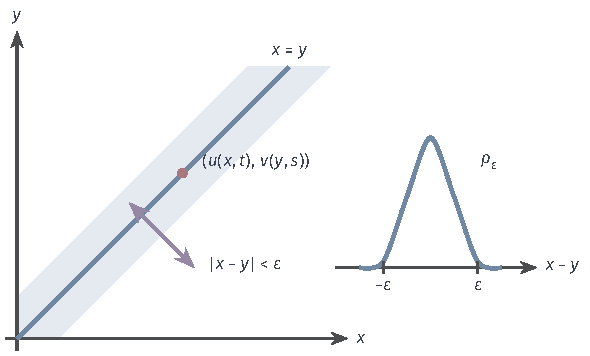
\includegraphics[width=99.9mm]{figures/06-differential-equations/02-partial-differential-equations/tikz/cons-doubling/figure.pdf}
  \caption{变量加倍的示意。左图是$(x,y)$平面（时间变量同理），两个解在两组独立变量上取值，浅蓝带是权重集中的区域，宽度约为$\varepsilon$。右图是横截面上的磨光核$\rho_\varepsilon$。令$\varepsilon\to0$，积分被压回对角线$x=y$。}
  \label{fig:cons-doubling}
\end{BookInlineFigure}

\begin{proof}
记$q(a,b)=\operatorname{sgn}(a-b)(F(a)-F(b))$。它关于$a,b$对称，并且当$\lvert a\rvert,\lvert b\rvert\leq M$时，
\[
  \lvert q(a,b)\rvert\leq L\,\lvert a-b\rvert .
\]

第一步，变量加倍。设$\phi(x,t,y,s)\geq0$是$(\mathbb{R}\times(0,\infty))^2$上的紧支光滑函数。固定$(y,s)$，在式~\eqref{eq:cons-kruzhkov}中对$u$取$k=v(y,s)$，再对$(y,s)$积分。类似地固定$(x,t)$，对$v$取$k=u(x,t)$，对$(x,t)$积分。两式相加，由$q$的对称性，
\[
  \iiiint\Bigl(\lvert u-v\rvert\,(\partial_t\phi+\partial_s\phi)
  +q(u,v)\,(\partial_x\phi+\partial_y\phi)\Bigr)\,\mathrm{d}x\,\mathrm{d}t\,\mathrm{d}y\,\mathrm{d}s\geq0 ,
\]
其中$u=u(x,t)$，$v=v(y,s)$。

第二步，选取测试函数。取非负$\psi\in C_c^{\infty}(\mathbb{R}\times(0,\infty))$和偶的标准磨光核$\rho_\varepsilon$，令
\[
  \phi=\psi\Bigl(\frac{x+y}{2},\frac{t+s}{2}\Bigr)\,
  \rho_\varepsilon\Bigl(\frac{x-y}{2}\Bigr)\,\rho_\varepsilon\Bigl(\frac{t-s}{2}\Bigr).
\]

求$\partial_t\phi+\partial_s\phi$时，$\rho_\varepsilon((t-s)/2)$的两项导数互相抵消，只剩$\psi$对时间的导数，空间变量同样。第一步的不等式化为
\[
  \iiiint\Bigl(\lvert u-v\rvert\,\partial_T\psi+q(u,v)\,\partial_X\psi\Bigr)\rho_\varepsilon\rho_\varepsilon\,\mathrm{d}x\,\mathrm{d}t\,\mathrm{d}y\,\mathrm{d}s\geq0 ,
\]
其中$\partial_T\psi,\partial_X\psi$在中点取值。

第三步，令$\varepsilon\to0$。作变量替换$X=(x+y)/2$，$\xi=(x-y)/2$，$T'=(t+s)/2$，$\tau=(t-s)/2$，Jacobian给出常数因子$4$。$\lvert a-b\rvert$与$q(a,b)$关于$a,b$是Lipschitz的，所以被积函数与其$\xi=\tau=0$时的值之差，被
\[
  C\bigl(\lvert u(X+\xi,T'+\tau)-u(X,T')\rvert+\lvert v(X-\xi,T'-\tau)-v(X,T')\rvert\bigr)
\]
控制。有界函数的平移在$L^1_{\mathrm{loc}}$中连续，这一项的积分在$\varepsilon\to0$时趋于零。于是对所有非负的$\psi$，
\begin{equation}
  \int_0^{\infty}\!\!\int_{\mathbb{R}}\Bigl(\lvert u-v\rvert\,\partial_t\psi+q(u,v)\,\partial_x\psi\Bigr)\,\mathrm{d}x\,\mathrm{d}t\geq0 .
  \label{eq:cons-kato}
\end{equation}

第四步，切出梯形。取$\delta\in(0,R)$和光滑不减函数$H_\delta$，$H_\delta(z)=0$（$z\leq-\delta$），$H_\delta(z)=1$（$z\geq0$）。取$\theta\in C_c^{\infty}(0,T)$，$\theta\geq0$，令
\[
  \psi(x,t)=\theta(t)\,\chi_\delta(x,t),\qquad
  \chi_\delta=1-H_\delta\bigl(\lvert x\rvert+L(t-T)-R\bigr).
\]
在$x=0$附近$H_\delta$的自变量小于$-\delta$，所以$\lvert x\rvert$的不光滑不影响$\psi$的光滑性。

记$H_\delta'$在上述自变量处取值，计算得
\[
  \partial_t\psi=\theta'\chi_\delta-\theta L H_\delta',\qquad
  \partial_x\psi=-\theta\operatorname{sgn}(x)H_\delta' .
\]

代入式~\eqref{eq:cons-kato}，整理后得到
\[
  \int_0^{T}\theta'(t)\int_{\mathbb{R}}\chi_\delta\,\lvert u-v\rvert\,\mathrm{d}x\,\mathrm{d}t
  \geq\iint\theta\,H_\delta'\,\bigl(L\,\lvert u-v\rvert+\operatorname{sgn}(x)\,q(u,v)\bigr)\,\mathrm{d}x\,\mathrm{d}t .
\]

$H_\delta'\geq0$，又由$\lvert q\rvert\leq L\lvert u-v\rvert$，右端非负。这一步是全部证明的关键：侧边的收缩速度$L$压过了流出的通量。

第五步，取极限。令$\delta\to0$，记
\[
  m(t)=\int_{\lvert x\rvert<R+L(T-t)}\lvert u(x,t)-v(x,t)\rvert\,\mathrm{d}x ,
\]
上面的不等式变成$\int_0^T\theta'(t)\,m(t)\,\mathrm{d}t\geq0$对所有非负的$\theta$成立。这说明$m$的弱导数非正，$m$几乎处处等于一个不增函数。

由式~\eqref{eq:cons-entropy-initial}，$t\downarrow0$时$m(t)$的本性极限是$\int_{\lvert x\rvert<R+LT}\lvert u_0-v_0\rvert\,\mathrm{d}x$。于是对几乎处处的$t\in(0,T)$，
\[
  \int_{\lvert x\rvert<R+L(T-t)}\lvert u-v\rvert\,\mathrm{d}x
  \leq\int_{\lvert x\rvert<R+LT}\lvert u_0-v_0\rvert\,\mathrm{d}x .
\]

令$R'=R+L(T-t)$，右端的半径就是$R'+Lt$，这正是要证的形式。让$(R,T)$取遍有理数，两端关于半径连续，所以结论对几乎处处的$t$和所有半径成立。
\end{proof}

证明中的两个地方用到了本章的条件。第一步的$k$可以取任意值，这需要Kruzhkov熵对所有$k$成立，只满足个别几个熵不够。第四步的$\lvert q\rvert\leq L\lvert u-v\rvert$需要$F$在解的取值范围内Lipschitz，这就是通量正则性与解有界的作用。

\paragraph{唯一性、收缩与比较}
把定理~\ref{thm:cons-contraction}用到不同的情形，就得到下面三条结论。比较原理需要把证明中的绝对值换成正部，做法很短，写在证明里。

\begin{theorem}[熵解的唯一性与稳定性]
\label{thm:cons-uniqueness}
在定理~\ref{thm:cons-contraction}的条件下：
\begin{enumerate}
  \item 若$u_0=v_0$几乎处处成立，则$u=v$几乎处处成立，即熵解唯一。
  \item 若$u_0-v_0\in L^1(\mathbb{R})$，则对几乎处处的$t>0$，
  \begin{equation}
    \lVert u(\cdot,t)-v(\cdot,t)\rVert_{1}\leq\lVert u_0-v_0\rVert_{1}.
    \label{eq:cons-l1-contraction}
  \end{equation}
  \item 若$u_0\leq v_0$几乎处处成立，则$u\leq v$几乎处处成立。特别地，$u$的值不超出$u_0$的本性下确界与本性上确界。
\end{enumerate}
\end{theorem}

\begin{proof}
第一条：式~\eqref{eq:cons-local-contraction}的右端为零。

第二条：在式~\eqref{eq:cons-local-contraction}中令$R\to\infty$。

第三条：$(u-k)^{+}$是凸函数，记$\operatorname{sgn}^{+}(z)$在$z>0$时为$1$，否则为$0$，与之配对的熵通量是$\operatorname{sgn}^{+}(u-k)(F(u)-F(k))$；$(k-v)^{+}$也是凸函数，熵通量是$\operatorname{sgn}^{+}(k-v)(F(k)-F(v))$。它们都是$C^2$凸熵的极限，所以各自满足式~\eqref{eq:cons-entropy-ineq}。

在变量加倍中，对$u$用前者并取$k=v(y,s)$，对$v$用后者并取$k=u(x,t)$，两式的被积函数相同，都是$(u-v)^{+}$和$\operatorname{sgn}^{+}(u-v)(F(u)-F(v))$。后者的绝对值同样不超过$L(u-v)^{+}$，所以第二步到第五步逐字照搬，得到
\[
  \int_{-R}^{R}(u-v)^{+}(x,T)\,\mathrm{d}x
  \leq\int_{-R-LT}^{R+LT}(u_0-v_0)^{+}\,\mathrm{d}x .
\]
$u_0\leq v_0$时右端为零，所以$u\leq v$。

常数是方程的熵解，取$v\equiv\operatorname*{ess\,sup}u_0$和$u\equiv\operatorname*{ess\,inf}u_0$作比较，得到值域的结论。
\end{proof}

第二条要求$u_0-v_0$可积，并不要求$u_0$、$v_0$本身可积。第一条和第三条不需要可积性，因为定理~\ref{thm:cons-contraction}是局部的，这正是有限传播速度的好处。阶跃初值不可积，但它和另一个只在有界区间上不同的初值之差可积，式~\eqref{eq:cons-l1-contraction}对它们仍然适用，式~\eqref{eq:cons-merge-distance}就是这样的例子。

存在性没有在这里证明。结论是：$F\in C^1$、$u_0\in L^{\infty}$时，熵解在$\mathbb{R}\times(0,\infty)$上存在且唯一。证明可以由消失黏性或单调差分格式的极限得到，需要一致的有界性和全变差估计，篇幅较长，读者可查阅前面提到的文献。本节的贡献是后半部分：极限至多只有一个，且连续依赖于初值。

\paragraph{收缩的两个推论}
收缩给出了比唯一性更多的信息。设$u_0$的全变差$\mathrm{TV}(u_0)$有限。方程不依赖$x$，所以平移$u(\cdot+h,\cdot)$也是熵解，由式~\eqref{eq:cons-l1-contraction}，
\[
  \lVert u(\cdot+h,t)-u(\cdot,t)\rVert_1\leq\lVert u_0(\cdot+h)-u_0\rVert_1\leq\lvert h\rvert\,\mathrm{TV}(u_0).
\]
除以$\lvert h\rvert$再令$h\to0$，得到$\mathrm{TV}(u(\cdot,t))\leq\mathrm{TV}(u_0)$。熵解不会产生新的振荡。

另一方面，式~\eqref{eq:cons-merge-distance}中的距离在有限时间内变成了零，所以时刻$t=1$的解不能告诉我们初值是斜坡还是阶跃。激波把特征线汇入后就丢掉了它们携带的信息。这个收缩是单向的：时间反演后距离可以增大，所以逆时间的问题不适定。

\paragraph{结论的边界}
这些结论只针对标量方程。系统的情形没有与式~\eqref{eq:cons-l1-contraction}对应的$L^1$收缩，也没有足够多的凸熵来运行变量加倍。已知的系统解理论需要初值全变差较小等附加条件，用的是不同的稳定性泛函。所以本节的结论不能直接移植到守恒律系统。


\section{本章小结}
\label{sec:cons-summary}

本章从车流的收支平衡出发，研究传播速度依赖未知量时会发生什么。特征线是直线，斜率由初值决定；只要相邻特征线的速度差使$1+a't$为零，斜率就在有限时间发散。此后解的值仍然有界，但$C^1$解不再存在，初值~\eqref{eq:cons-bump}的破裂时刻是$T^{*}=8\sqrt{3}/9$，斜坡~\eqref{eq:cons-ramp}的破裂时刻是$T^{*}=1$。

收支平衡不依赖导数，于是弱形式~\eqref{eq:cons-weak}接纳了间断，Rankine--Hugoniot条件~\eqref{eq:cons-rh}把间断的速度变成了通量的弦斜率。但这只是总量守恒的要求。同一阶跃初值有一整族弱解~\eqref{eq:cons-weak-family}，零初值也有非零的弱解~\eqref{eq:cons-zero-data}，守恒本身选不出解。

熵条件补上了这一步。从特征线看，它要求特征线汇入间断；从小黏性看，它是黏性耗散在极限中留下的不等式；从通量图像看，它是弦与图像的上下关系。Riemann问题把这些条件落实为计算：严格凸通量下，$u_l>u_r$得到激波，$u_l<u_r$得到稀疏波。表~\ref{tab:cons-summary}把各个解的概念放在一起。

\begin{BookInlineTable}
  \centering
  \caption{标量守恒律的解的概念及其适用条件。}
  \label{tab:cons-summary}
  \begin{tabular}{p{16mm}p{32mm}p{24mm}p{20mm}}
    \toprule
    概念 & 要求 & 存在范围 & 唯一性\\
    \midrule
    $C^1$解 & 逐点满足方程 & 到$T^{*}$为止 & 有\\
    弱解 & 式~\eqref{eq:cons-weak}，间断满足跳跃条件 & 整体（含熵解） & 无\\
    熵解 & 弱解加所有凸熵不等式 & 整体，$u_0\in L^{\infty}$ & 有，且$L^1$收缩\\
    \bottomrule
  \end{tabular}
\end{BookInlineTable}

最后，变量加倍把熵不等式变成两个熵解之间的比较，给出局部$L^1$收缩~\eqref{eq:cons-local-contraction}，由此得到唯一性、比较原理和全变差不增。这些结论依赖通量的正则性和解的有界性，$L^1$距离还要求初值之差可积；存在性依赖消失黏性或差分格式的极限，本章未证。一维标量以外的情形，尤其是守恒律系统，不能照搬这些结论。

守恒和正确的解选择缺一不可：只有守恒，解太多；只有特征线，解在相交之后不存在。第~\ref{chap:pde-numerical-methods}章的有限体积方法在每个单元界面上解一个Riemann问题，复用的正是这里的局部传播结构。

